% !TeX root = presentation.tex
% !TeX program = xelatex
% ============================================================
%  Potential-Based Reward Shaping for Planar Pushing
%  Single-Agent Control vs Asymmetric Self-Play
%  Master Thesis Presentation — 30 minutes, 16:9
%  Theme: SimplePlusAIC (requires XeLaTeX or LuaLaTeX)
% ============================================================
\PassOptionsToPackage{table,dvipsnames}{xcolor}
\documentclass[aspectratio=169,xcolor=dvipsnames,t]{beamer}
\usepackage{fontspec}  % REQUIRED before theme for Epilogue font
\usepackage{colortbl}  % required for \rowcolor in tables
\usetheme{SimplePlusAIC}

\usepackage{amsmath,amssymb,amsfonts}
\usepackage{bm}
\usepackage{graphicx}
\usepackage{booktabs}
\usepackage{multirow}
\usepackage{tikz}
\usetikzlibrary{positioning,arrows.meta}
\usepackage{hyperref}

% --- Override AIC logo (not applicable to University of Groningen) ---
\logo{}

% --- Clean footline (institute removed; already on title slide; avoids \litfooter collisions) ---
\setbeamertemplate{footline}{%
  \begin{beamercolorbox}[ht=2em,sep=0.75em,wd=\paperwidth,leftskip=0.5cm,rightskip=0.5cm]{footlinecolor}
    \hfill
    \scriptsize{\insertframenumber}
  \end{beamercolorbox}%
}

% --- Custom colors (complementary to theme's Bordeaux/DarkBordeaux/Astronaut) ---
\definecolor{hlblue}{RGB}{0,102,204}
\definecolor{hlgreen}{RGB}{0,140,60}
\definecolor{hlred}{RGB}{190,30,30}
\definecolor{lightgray}{RGB}{220,220,220}

% --- Literature footer ---
\newcommand{\litfooter}[1]{%
  \vspace{2pt}%
  \hrule%
  \vspace{2pt}%
  {\tiny\color{LightDarkGrey} #1}%
}

% --- Full-bleed image frame (plain, no title/footer) ---
\newcommand{\fullbleedframe}[1]{%
  \begin{frame}[plain]
    \centering
    \includegraphics[width=\paperwidth,height=\paperheight,keepaspectratio]{#1}%
  \end{frame}%
}

% --- Media box: show image if present, else a labeled placeholder ---
% #1 = width fraction of \textwidth, #2 = file name in figures/
\newcommand{\mediabox}[2]{%
  \IfFileExists{figures/#2}{%
    \includegraphics[width=#1\textwidth]{figures/#2}%
  }{%
    \setlength{\fboxsep}{6pt}%
    \fcolorbox{LightDarkGrey}{lightgray}{%
      \begin{minipage}[c][0.26\textheight][c]{#1\textwidth}%
        \centering\small\itshape [clip placeholder]\\[3pt]
        \texttt{\footnotesize \detokenize{figures/#2}}\\[3pt]record \& drop file here%
      \end{minipage}%
    }%
  }%
}

% --- Clickable "play clip" link (works in Okular / Adobe via run:) ---
\newcommand{\playclip}[1]{\href{run:figures/#1}{\scriptsize\color{hlblue}$\blacktriangleright$ play clip}}

% --- Title info ---
\title[PBRS for Planar Pushing]{Potential-Based Reward Shaping \\for Planar Pushing}
\subtitle{Single-Agent Control vs.\ Asymmetric Self-Play}
\author{Vlad Iftime s3426394}
\institute[University of Groningen, FSE]{Faculty of Science and Engineering, Artificial Intelligence \\ University of Groningen}
\date{June 2026}

% --- Final page text ---
\finalpagetext{Thank You — Questions?}

\begin{document}

% ============================================================
% TITLE PAGE (theme macro)
% ============================================================
\addtobeamertemplate{title page}{\vspace{-14pt}}{}
\maketitlepage

% ~~~~~ SPEAKER NOTES ~~~~~
\note[itemize]{
\item 30-minute master thesis presentation
\item Topic: potential-based reward shaping for planar pushing with a UR5e robot arm
\item 8 model variants: PBRS single-agent through time-based ASP
\item Key result: simplest model (PBRS single-agent, 80.0\%) beats every structured variant
\item Curriculum and self-play degrade performance; reward and curriculum are independent levers
}

% ============================================================
% SLIDE 0 — OVERVIEW
% ============================================================
\begin{frame}[t]{Overview — Thesis Structure}
  \vspace*{-0.35cm}
  \footnotesize
  \begin{columns}[T,onlytextwidth]
    \begin{column}{0.24\textwidth}
      {\textbf{\color{hlblue}1.\ \ The Problem}}
      \begin{itemize}
        \item MDP Formulation
        \item Push Mechanics \\ (Limit Surface)
        \item Old Ad-hoc Reward \\ Failure
      \end{itemize}
    \end{column}
    \begin{column}{0.24\textwidth}
      {\textbf{\color{hlblue}2.\ \ PBRS Solution}}
      \begin{itemize}
        \item PBRS Theory
        \item Potential Functions
        \item SE(2) Unified \\ Distance Metric
      \end{itemize}
    \end{column}
    \begin{column}{0.24\textwidth}
      {\textbf{\color{hlblue}3.\ \ What We Built}}
      \begin{itemize}
        \item \textbf{A}: PBRS Single-Agent
        \item \textbf{B}: Forced Curriculum
        \item \textbf{C–D}: ASP (Alice/Bob)
        \item \textbf{E–H}: ASP Variants \\ (SE(2), disc, time-based)
      \end{itemize}
    \end{column}
    \begin{column}{0.24\textwidth}
      {\textbf{\color{hlgreen}4.\ \ What We Found}}
      \begin{itemize}
        \item PBRS outperforms \\ ad-hoc reward
        \item ASP severely \\ underperforms
        \item Reward and curriculum \\ are independent
        \item Simplest model wins \\ every time
      \end{itemize}
    \end{column}
  \end{columns}
\end{frame}

% ~~~~~ SPEAKER NOTES ~~~~~
\note[itemize]{
\item Roadmap — four stages, left to right
\item Stage 1 — Planar Pushing MDP: task definition, quasi-static push mechanics (limit surface), SE(2) distance metric
\item Stage 2 — PBRS Theory: why the ad-hoc reward failed, the shaping theorem, our exponential potential functions
\item Stage 3 — 8 Model Variants: A (single-agent PBRS), B (curriculum), C–H (ASP / Alice-Bob, 6 variants)
\item Stage 4 — Key Findings: why ASP fails, reward–curriculum independence, computational overhead, unified comparison
}

% ============================================================
% SLIDE 1 — RESEARCH QUESTIONS
% ============================================================
\begin{frame}[t]{Research Questions}
  \begin{block}{Three Research Questions}
    \begin{enumerate}
      \item \textbf{RQ1:} Can potential-based reward shaping replace hand-tuned dense rewards for planar pushing tasks?
      \item \textbf{RQ2:} Does curriculum learning or asymmetric self-play improve sample efficiency over a direct single-agent approach?
      \item \textbf{RQ3:} Are reward design and curriculum design \emph{independent} problems in contact-rich manipulation?
    \end{enumerate}
  \end{block}

  \vspace{2pt}
  \vfill\litfooter{[Ng, Harada \& Russell 1999]~\textbf{[Grze\'s 2017]}~[Devlin \& Kudenko 2012]}
\end{frame}

% ~~~~~ SPEAKER NOTES ~~~~~
\note[itemize]{
\item RQ1: Yes — Model A achieves 80\% validation SR on 30 held-out T-block scenes
\item RQ2: No — curriculum (B, 76.7\%) and ASP (E–H, 6.7–16.7\%) underperform single-agent
\item RQ3: Yes — the 2×2 ablation shows reward and curriculum are independent levers
\item 8 models, {\textasciitilde}3000 iterations each, 528 parallel environments, RTX Pro 6000
}

% ============================================================
% SLIDE 2 — MDP FORMULATION
% ============================================================
\begin{frame}[t]{MDP Formulation — State \& Action}
  \begin{columns}[T]
    \begin{column}{0.58\textwidth}
      \textbf{State} $\mathbf{s} \in \mathbb{R}^{28}$: \\[2pt]
      {\small $\mathbf{s} = [\;\underbrace{\mathbf{q}_{\text{ee}}}_{\text{EE pose}(6)}\;|\;
        \underbrace{\mathbf{p}_{\text{obj}}, \mathbf{R}_{\text{obj}}}_{\text{obj state}(14)}\;|\;
        \underbrace{\mathbf{p}_{\text{goal}}, \mathbf{R}_{\text{goal}}}_{\text{goal pose}(6)}\;|\;
        \underbrace{d_{\text{pos}}, d_{\text{rot}}}_{\text{errors}(2)}\;]$}

      \vspace{4pt}
      \textbf{Action} $\mathbf{a} \in \mathbb{R}^4$ (object-relative): \\[2pt]
      {\small $(r,\phi,\ell,\theta)$ with 21 bins/dim $\Rightarrow$ 194\,481 discrete actions}
      \[
      \begin{aligned}
      X_s &= x_{\text{obj}} + r \cos(\psi_{\text{obj}} + \phi) \\
      Y_s &= y_{\text{obj}} + r \sin(\psi_{\text{obj}} + \phi) \\
      X_f &= X_s + \ell \cos\theta,\quad Y_f = Y_s + \ell \sin\theta
      \end{aligned}
      \]
    \end{column}
    \begin{column}{0.38\textwidth}
      \centering
      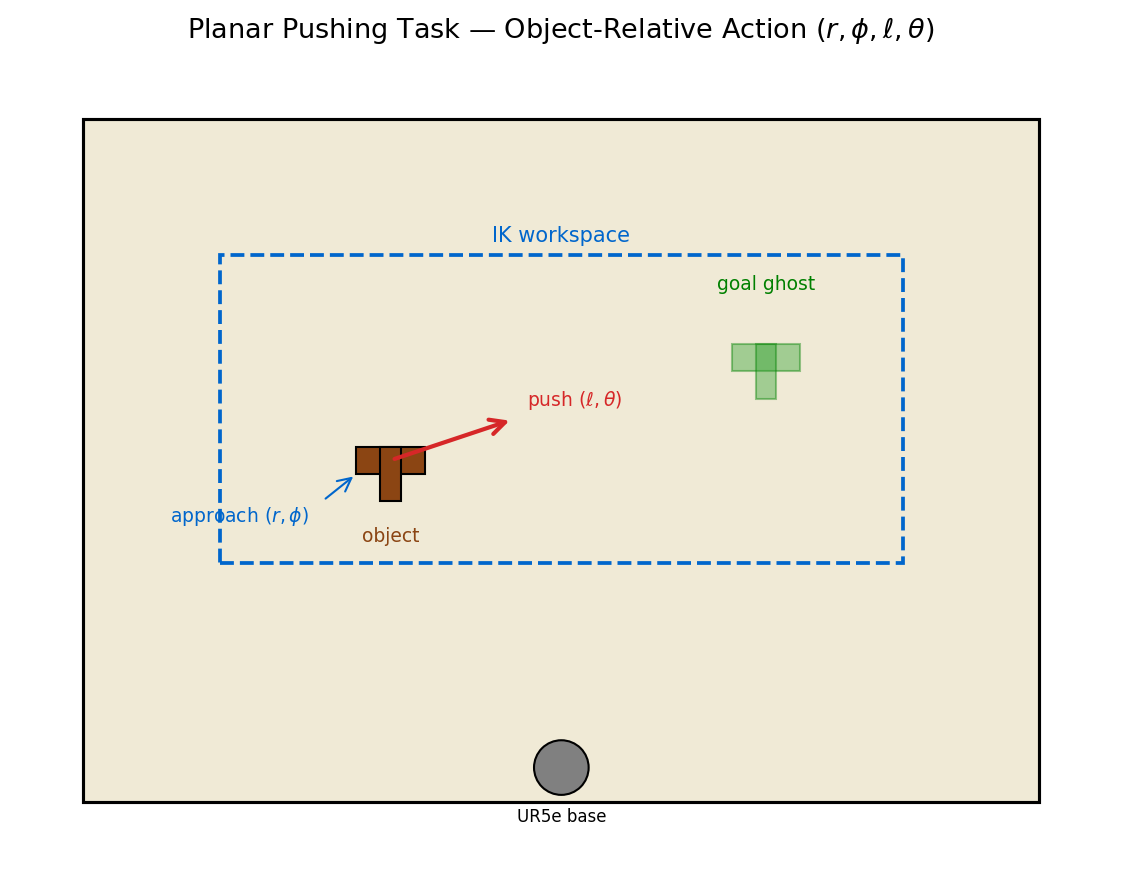
\includegraphics[width=1.0\textwidth]{figures/diagram_task_schematic.png}
      \vspace{2pt}
    \end{column}
  \end{columns}

  \vfill\litfooter{[Mason 1986]~[Lynch \& Mason 1996]~[Goyal et al.\ 1991]}
\end{frame}

% ~~~~~ SPEAKER NOTES ~~~~~
\note[itemize]{
\item The MDP is a planar pushing task: a UR5e robot pushes a T-block or disc object on a 1.4m × 1.0m table
\item State is 28D: end-effector pose (6), object state including position and quaternion (14), goal pose (6), and current distance errors (2)
\item Action is 4D macro-parameterized as object-relative approach (r, phi) plus world-frame push direction (length, theta). 21 bins per dimension = 194k discrete actions
\item Object-relative actions are critical — they guarantee ~95\% contact rate regardless of object spawn position, vs ~2\% for absolute coordinates
}

% ============================================================
% SLIDE 2b — MDP: TRANSITION & EPISODE
% ============================================================
\begin{frame}[t]{MDP Formulation — Transition \& Episode}
  \small
  \textbf{Transition — quasi-static limit surface} (Mason 1986): $\mathbf{t} = (v_x, v_y, \omega) \propto \nabla f(\mathbf{w})$. Object twist is normal to the surface — every push couples translation \emph{and} rotation.

  \vspace{4pt}
  \textbf{Episode (training):} max 15 pushes; \textbf{Validation:} 30 pushes, best-of-20 retries.

  \textbf{Success:} pos $<$ 5\,cm \textbf{and} rot $<$ 0.2\,rad.  Ends early on catastrophe (tipped / launched / OOB).  Table $1.40\times1.00$\,m; IK $X\!\in\![-0.5,0.5]$, $Y\!\in\![0.25,0.70]$\,m.

  \vfill\litfooter{[Mason 1986]~[Lynch \& Mason 1996]~[Goyal et al.\ 1991]}
\end{frame}

% ~~~~~ SPEAKER NOTES ~~~~~
\note[itemize]{
\item Transition: quasi-static limit-surface normality theorem — every push couples translation and rotation via the surface gradient
\item Episode: 15 pushes training; validation uses 30 pushes with best-of-20 retries. Success = pos < 5cm AND rot < 0.2 rad
\item Table 1.40m × 1.00m; IK workspace X∈[−0.50,0.50], Y∈[0.25,0.70]
}
% Slide 3a moved to appendix (Push Mechanics — Limit Surface + L)
% ============================================================


% ============================================================
% SLIDE 3b — SE(2) UNIFIED DISTANCE
% ============================================================
\begin{frame}[t]{SE(2) Unified Distance — Models E-H}
  \begin{columns}[T,onlytextwidth]
    \begin{column}{0.54\textwidth}
      \textbf{SE(2) metric:} $d_{\text{pose}} = \sqrt{dx^2 + dy^2 + L^2 d\theta^2}$
      \begin{itemize}
        \item Single scalar combining $(dx,dy)$ and $d\theta$; $L$ = char.\ length (T-block $0.07$m, disc $0$m)
        \item \textbf{Single-potential PBRS:} $\Phi(s)=w\,e^{-k\,d_{\text{pose}}^2}$, $k=30,\,w=10$
        \item Eliminates competing pos/rot gradients — aligns reward with the coupled physics
      \end{itemize}
      \textbf{Result:} SE(2) does \emph{not} rescue ASP — E/F reach only 6.7\% validation SR vs single-agent 80\%. The self-play curriculum is the root cause, not the metric.
    \end{column}
    \begin{column}{0.44\textwidth}
      \centering
      
\includegraphics[width=1.0\textwidth]{figures/diagram_limit_surface.png}
    \end{column}
  \end{columns}

  \vfill\litfooter{[Park 1995]~[Urain et al.\ 2023]~[Lynch \& Mason 1996]}
\end{frame}

% ~~~~~ SPEAKER NOTES ~~~~~
\note[itemize]{
\item The SE(2) unified distance replaces separate position and rotation errors with a single Riemannian metric on the planar rigid-body configuration space
\item L converts radians to meters. For the T-block with L=0.07m, 0.5 rad of rotation contributes 3.5cm to d_pose — roughly equal weight with a 3.5cm position displacement
\item For the disc with L=0m, rotation is irrelevant — d_pose collapses to pure position distance, matching the physical symmetry
\item The single-potential PBRS eliminates the competing gradient problem: separate pos/rot potentials each pull in different directions, while the SE(2) potential provides a unified gradient
\item Both Model E (SE(2) d_pose ASP) and Model C (separate ASP) collapse — the SE(2) metric doesn't rescue the self-play dynamics, confirming the curriculum is the root cause, not the reward metric
}

% ============================================================
% SLIDE 4 — OLD REWARD FORMULA FAILURE
% ============================================================
\begin{frame}[t]{Old Reward Formula — Why It Failed}
  \begin{block}{Fractional Improvement Formula (Fixes P63-P64)}
    \[
    R = \underbrace{\alpha\!\cdot\!\frac{d_{\text{prev}}\!-\!d_{\text{now}}}{d_{\text{prev}}}}_{\text{position improvement}}
        + \underbrace{\alpha\!\cdot\!\frac{y_{\text{prev}}\!-\!y_{\text{now}}}{y_{\text{prev}}}}_{\text{rotation improvement}}
        - \underbrace{\beta_{\text{pos}}\!\cdot\!d_{\text{now}}}_{\text{position penalty}}
        - \underbrace{\beta_{\text{rot}}\!\cdot\!y_{\text{now}}}_{\text{rotation penalty}}
    \]
    {\small $\alpha=3.0,\;\beta_{\text{pos}}=0.5,\;\beta_{\text{rot}}=0.25$\\
    $d_{\text{prev}},d_{\text{now}}$: position error before/after push;\; $y_{\text{prev}},y_{\text{now}}$: rotation error before/after push}
  \end{block}

  \vspace{-6pt}
  \begin{columns}[T]
    \begin{column}{0.50\textwidth}
      {\footnotesize \textbf{Problem 1 — Non-Markov:} Depends on $d_{\text{prev}}$ — same state transition gets different reward from different starting positions. Value function ill-defined.}
    \end{column}
    \begin{column}{0.46\textwidth}
      {\footnotesize \textbf{Problem 2 — Gradient Starvation:} 1cm improvement from 30cm: \textcolor{hlred}{$\alpha\!\cdot\!0.01/0.30 - \beta_{\text{pos}}\!\cdot\!0.29 = \mathbf{-0.045}$}. Progress gets $\mathbf{negative}$ reward. $\mathbb{E}[R] \approx -0.15$, near-zero variance.}
    \end{column}
  \end{columns}

  \vspace{-2pt}
  {\footnotesize \textbf{Result:} The fractional formula suffers from two structural flaws — non-Markov dependence and gradient starvation — making it fundamentally unsuitable for stable RL training.}

  \vfill\litfooter{[Ng et al.\ 1999]~[Grzes \& Kudenko 2009]}
\end{frame}

% ~~~~~ SPEAKER NOTES ~~~~~
\note[itemize]{
\item The old fractional improvement formula had two fatal flaws
\item First, it's non-Markov: dividing by d_prev makes reward depend on starting position. The same state transition gets different reward. I prove in my thesis appendix that no static potential Phi(s) can reproduce this reward
\item Second, gradient starvation: a push producing genuine progress gets penalized because the penalty term dominates. The expected reward for random pushes is negative with near-zero variance — PPO's GAE gets no signal to differentiate good from bad pushes
\item This is WHY we needed a better reward function — PBRS fixes both problems
}

% ============================================================
% SLIDE 5a — PBRS THEOREM + POTENTIALS
% ============================================================
\begin{frame}[t]{PBRS — The Shaping Theorem}
  \textbf{Ng et al.\ (1999):}
  \[
  \boxed{\mathcal{R}'(s,a,s') = \mathcal{R}(s,a,s') + \underbrace{\gamma\Phi(s') - \Phi(s)}_{\text{shaping reward }F}}
  \]
  \textbf{Policy invariance:} $Q'(s,a) = Q(s,a) - \Phi(s)$ — optimal actions unchanged.

  \vspace{4pt}
  \textbf{Our potential functions (Models A/B):}
  \[
  \Phi(s) = w_{\text{pos}} e^{-k_p d_{\text{pos}}^2} + w_{\text{rot}} e^{-k_r c(s)},\quad
  c(s) = \frac{1-\cos(\theta^*-\theta)}{2}
  \]
  $k_p{=}30,\; k_r{=}5,\; w_{\text{pos}}{=}w_{\text{rot}}{=}10.0$\\
  \textbf{Dense reward:} $F(s,s') = \Phi(s') - \Phi(s)$  —  difference only, no constant drain.

  \vspace{4pt}
  \textbf{Episodic PBRS} (Grze\'s 2017): $\gamma_{\text{shaping}}{=}1.0$ valid — $\sum F = \Phi(s_T)-\Phi(s_0)$ bounded.

  \vfill\litfooter{[Ng, Harada \& Russell 1999]~\textbf{[Grze\'s 2017]}~[Devlin \& Kudenko 2012]}
\end{frame}

% ~~~~~ SPEAKER NOTES ~~~~~
\note[itemize]{
\item The fundamental theorem: add F = gamma·Phi(s') − Phi(s) without changing optimal policies
\item Proof sketch: Q'(s,a) = Q(s,a) − Phi(s). Since Phi(s) depends on state only (not action), argmax unchanged
\item Our potential: sum of two exponentiated distance functions. Cosine c(s) respects S¹ topology — no discontinuity at ±π
\item Episodic PBRS: gamma_shaping=1.0 is valid — sum over an episode is bounded = Phi(s_T) − Phi(s_0)
}

% ============================================================
% SLIDE 5a-ii — WHY PBRS IS IDEAL FOR PLANAR PUSHING
% ============================================================
\begin{frame}[t]{PBRS — Why It's the Right Choice for Planar Pushing}
  \textbf{Properties of $F(s,s') = \Phi(s') - \Phi(s)$:}
  \begin{enumerate}
    \item \textbf{Markovian} — depends only on $s,s'$, not history. Old formula violated this by dividing by $d_{\text{prev}}$.
    \item \textbf{Bounded} — exponential potentials prevent reward explosions from PhysX contact spikes.
    \item \textbf{Zero-sum cycles} — detour pushes net to zero; agent free to explore without reward hacking.
    \item \textbf{No constant drain} — $F{=}0$ when stationary; no penalty for hesitation or deliberation.
  \end{enumerate}

  \vspace{4pt}
  \textbf{Key consequence:} you can replace any ad-hoc reward with a potential-based one \emph{without changing what the agent learns} — only \emph{how fast} it learns. Reward design and policy optimisation are decoupled.

  \vfill\litfooter{[Ng, Harada \& Russell 1999]~\textbf{[Grze\'s 2017]}~[Harutyunyan et al.\ 2015]}
\end{frame}

% ~~~~~ SPEAKER NOTES ~~~~~
\note[itemize]{
\item Four properties that make PBRS ideal for contact-rich pushing: Markovian (depends only on s,s'), Bounded (exponentials cap reward range), Zero-sum cycles (detour pushes give zero net F — no reward hacking), No constant drain (stationary agent gets F=0)
\item The old fractional improvement formula violated all four — non-Markov (divides by d_prev), unbounded (division by 0.01), negative-sum (staying still was penalised)
}

% ============================================================
% SLIDE 5b — PBRS REWARD ANALYSIS
% ============================================================
\begin{frame}[t]{PBRS — Reward Signal Analysis}
  \begin{columns}[T,onlytextwidth]
    \begin{column}{0.48\textwidth}
      \centering
      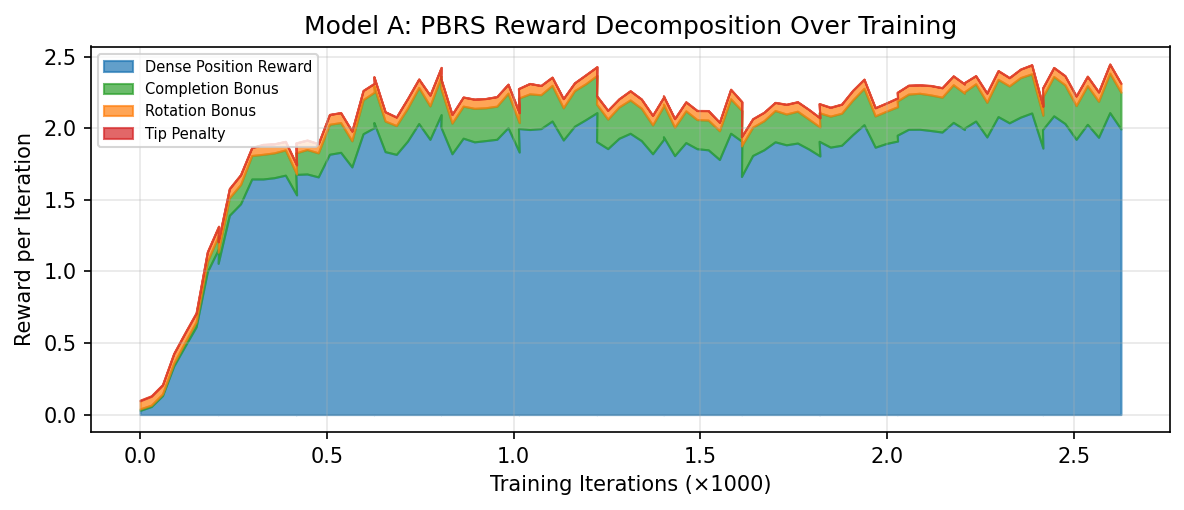
\includegraphics[width=1.0\textwidth]{figures/plot5_reward_diet.png}
      \vspace{2pt}
      {\footnotesize\textbf{Reward diet:} $\sim$85\% dense PBRS shaping,\\+5/+2 sparse bonuses, penalties.}
    \end{column}
    \begin{column}{0.48\textwidth}
      \centering
      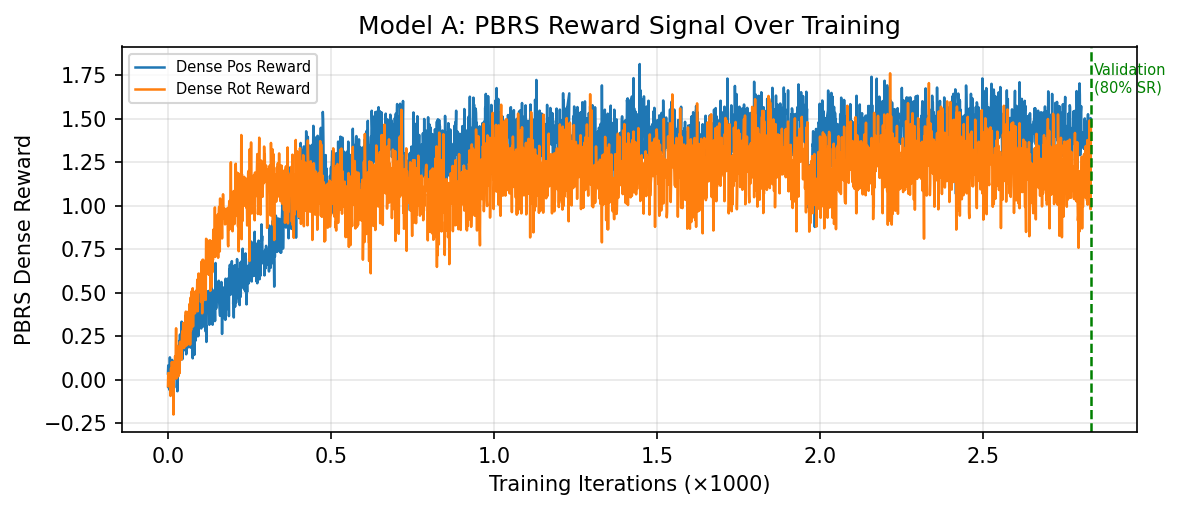
\includegraphics[width=1.0\textwidth]{figures/plot1_pbrs_signal_vs_performance.png}
      \vspace{2pt}
      {\footnotesize\textbf{Signal vs performance:} bounded exponential\\potentials $\to$ stable, correlated gradient.}
    \end{column}
  \end{columns}

  \vspace{4pt}
  {\small Dense signal on every push, bounded rewards, stable value — PBRS avoids the gradient starvation and critic instability of the old fractional formula.}

  \vfill\litfooter{[Ng, Harada \& Russell 1999]~\textbf{[Grze\'s 2017]}~[Harutyunyan et al.\ 2015]}
\end{frame}

% ~~~~~ SPEAKER NOTES ~~~~~
\note[itemize]{
\item Reward diet: $\sim$85\% of reward from dense PBRS shaping. Sparse completion bonuses (+5/+2) are supplementary — PPO always has a gradient to follow
\item Signal vs performance: the bounded exponential potentials produce a stable, correlated relationship between PBRS signal and training progress. The old fractional reward had near-zero variance (all pushes looked equally bad to GAE)
\item Cosine angular distance on rotation respects S¹ topology — no wrap-around discontinuity at ±π
}

% ============================================================
% SLIDE 6a — MODEL A: ARCHITECTURE + TRAINING
% ============================================================
\begin{frame}[t]{Model A — PBRS Single-Agent (Our Best Model)}
  \small
  \textbf{Architecture:} Single PPO agent, LSTM(28$\to$256) + MLP[512, 256] trunk, MultiCategorical head (4 dims $\times$ 21 bins). No curriculum, no Alice/Bob, no GoalEncoder.

  \textbf{Training:} 528 envs, 15 pushes/rollout, $\sim$3000 iterations $\sim$1.6 days wall-clock ($\sim$0.022 it/s).

  \textbf{Why it works:}
  \begin{enumerate}
    \item \textbf{Dense, bounded gradient} — PBRS fires on every push
    \item \textbf{Fixed goal distribution} — stationary random goals; no adversarial shift
    \item \textbf{Single network} — one agent, one optimizer; no multi-agent instability
  \end{enumerate}

  \vfill\litfooter{[Ng et al.\ 1999]~[Grze\'s 2017]~[Schulman et al.\ 2017]}
\end{frame}

% ~~~~~ SPEAKER NOTES ~~~~~
\note[itemize]{
\item Model A is the simplest possible architecture: single PPO agent with LSTM+MLP, PBRS reward, sparse completion bonuses
\item Three reasons it works: PBRS provides dense gradient at every push, fixed random goal distribution avoids adversarial shift, single network avoids multi-agent optimization instability
\item Converges within 1500 iterations. Stable value function bounded by exponential potentials
}

% ============================================================
% SLIDE 6b — MODEL A: TRAINING CURVES
% ============================================================
\begin{frame}[t]{Model A — Training Dynamics}
  \begin{center}
    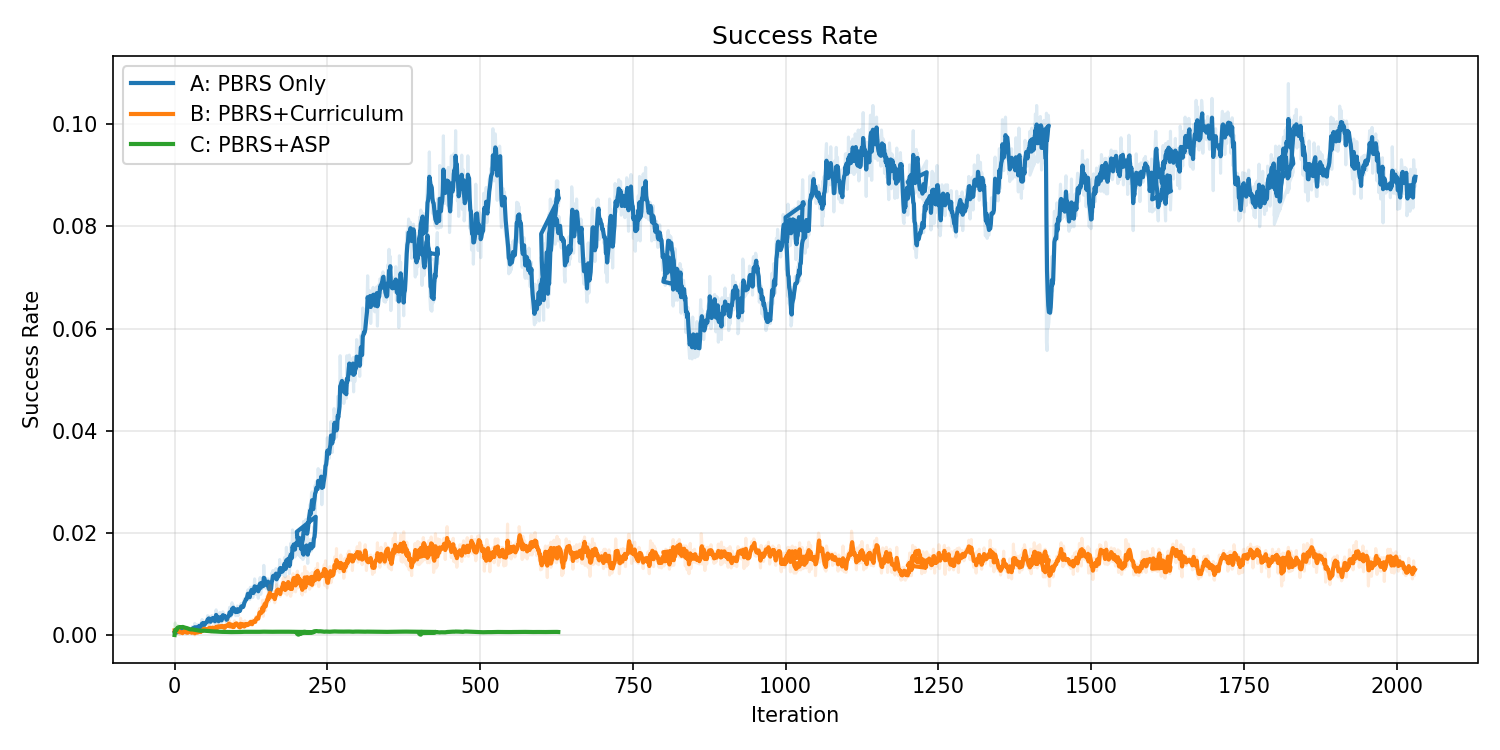
\includegraphics[width=0.48\textwidth]{figures/cmp_Success_Rate.png}
    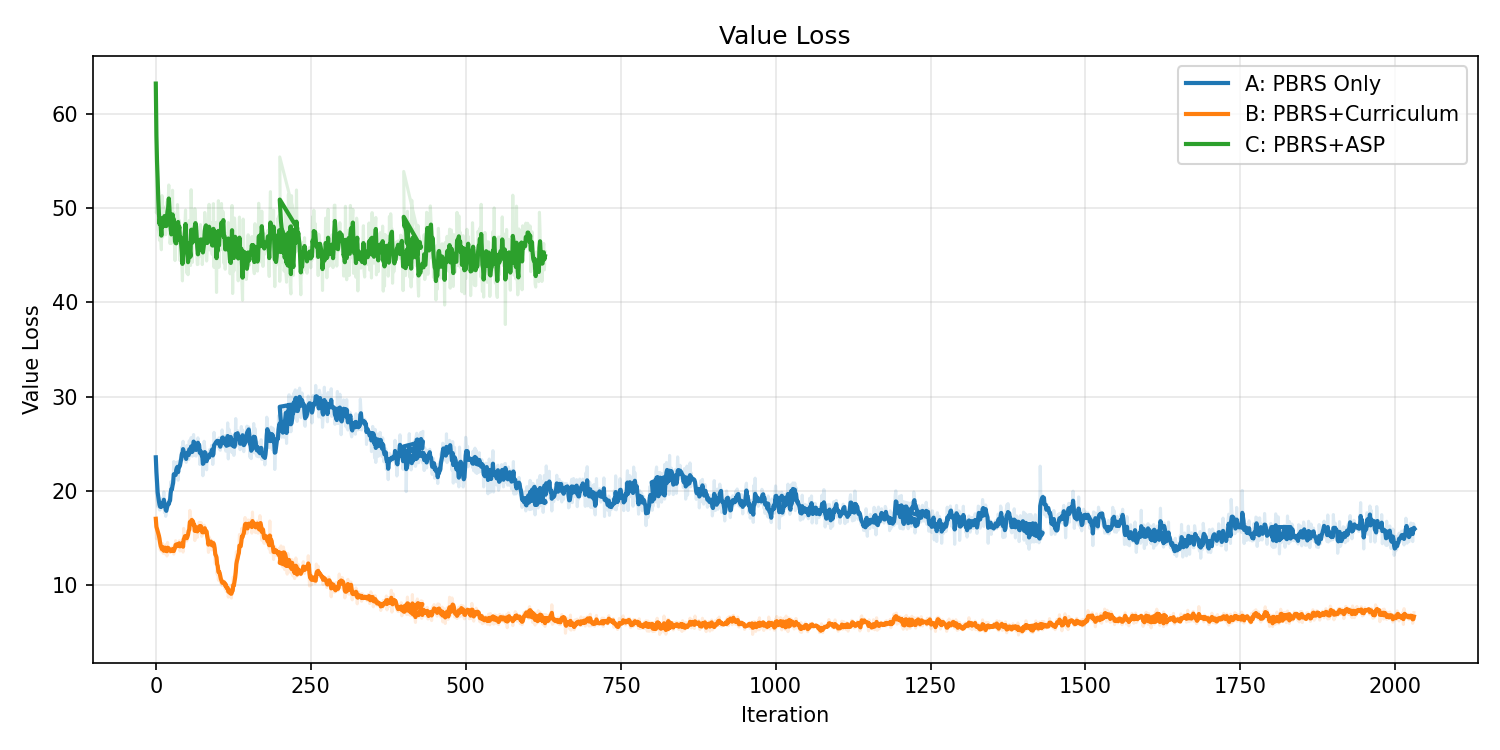
\includegraphics[width=0.48\textwidth]{figures/cmp_Value_Loss.png}
  \end{center}

  \vspace{2pt}
  {\small \textbf{Left:} Model A (blue) steadily improves training success rate over 3000 iterations. Model B (orange) follows a similar trajectory but converges slightly lower. ASP variants (E–H) remain near baseline throughout. \textbf{Right:} Stable value function — no explosion. Initial $V\approx0.057$ with gain$=0.01$.}

  \vfill\litfooter{[Schulman et al.\ 2017]~[Ng et al.\ 1999]}
\end{frame}

% ~~~~~ SPEAKER NOTES ~~~~~
\note[itemize]{
\item Left plot: training success rate over ~3000 iterations. Model A (blue) improves from near-zero to ~9.4\% (strict combined gate). Model B (orange, P82-fixed) follows a similar trajectory. ASP variants (E-H) remain near baseline
\item Right plot: value loss stays stable — no explosion. The PBRS exponential potentials prevent the reward spikes that caused GAE chain reactions and critic instability in earlier attempts
}

% ============================================================
% SLIDE 6c — MODEL A: VALIDATION RESULTS
% ============================================================
\begin{frame}[t]{Model A — Validation Results}
  \begin{columns}[T,onlytextwidth]
    \begin{column}{0.50\textwidth}
      \textbf{30 held-out T-block scenes (best-of-20):}
      \begin{itemize}
        \item \textcolor{hlgreen}{\textbf{80.0\% SR}} (24/30) — pos-only \textbf{100\%}, pos+rot \textbf{70\%}
        \item PosErr \textbf{0.032\,m}, RotErr \textbf{0.568\,rad}
        \item Training SR ($\sim$9.4\%) understates validation — strict combined gate vs best-of-20
      \end{itemize}
    \end{column}
    \begin{column}{0.48\textwidth}
      \centering
      \mediabox{1.0}{rec_push_s21_key.png}\\[2pt]
      {\scriptsize Overhead view — Model A solving a pos+rot scene}\quad\playclip{rec_push_s21.mp4}
    \end{column}
  \end{columns}

  \vfill\litfooter{[Ng et al.\ 1999]~[Grze\'s 2017]~[Schulman et al.\ 2017]}
\end{frame}

% ~~~~~ SPEAKER NOTES ~~~~~
\note[itemize]{
\item Validation: 30 held-out T-block scenes, best-of-20 protocol. 80.0\% overall SR
\item Perfect on position-only scenes (100\%), strong on combined pos+rot scenes (70\%)
\item PosErr 0.032m and RotErr 0.568 rad on successful episodes
\item Training SR (∼9.4\%) understates validation because the strict combined gate penalizes near-misses in training. Validation uses best-of-3/best-of-20 retries
\item The overhead clip shows the trained Model A policy recorded top-down
}

% ============================================================
% SLIDE 6c-i2 — MODEL A: VALIDATION RUNS (3-up overhead clips)
% ============================================================
\begin{frame}[t]{Model A — Validation Runs (overhead)}
  {\small Three held-out T-block scenes, top-down camera — the trained Model A policy:}

  \vspace{4pt}
  \begin{columns}[T,onlytextwidth]
    \begin{column}{0.32\textwidth}
      \centering
      \mediabox{1.0}{rec_push_s11_key.png}\\[2pt]
      {\scriptsize Forward (pos-only)}\quad\playclip{rec_push_s11.mp4}
    \end{column}
    \begin{column}{0.32\textwidth}
      \centering
      \mediabox{1.0}{rec_push_s14_key.png}\\[2pt]
      {\scriptsize Lateral push (pos-only)}\quad\playclip{rec_push_s14.mp4}
    \end{column}
    \begin{column}{0.32\textwidth}
      \centering
      \mediabox{1.0}{rec_push_s21_key.png}\\[2pt]
      {\scriptsize Translate + rotate}\quad\playclip{rec_push_s21.mp4}
    \end{column}
  \end{columns}

  \vfill\litfooter{[Ng et al.\ 1999]~[Grze\'s 2017]~[Schulman et al.\ 2017]}
\end{frame}

% ~~~~~ SPEAKER NOTES ~~~~~
\note[itemize]{
\item Three representative validation runs recorded top-down with record\_push\_video.py
\item Left: a short forward push (E\_Forward, position-only)
\item Middle: a lateral push (E\_Left, position-only)
\item Right: a combined translate-and-rotate scene (E\_Diag, position+rotation)
\item All use the same simple PBRS Model A checkpoint with object-relative obs+actions
}

% ============================================================
% SLIDE 6c-ii — ALL MODELS: VALIDATION WITH ERROR BARS
% ============================================================
\begin{frame}[t]{Multi-Model Validation — with Confidence Intervals}
  \begin{columns}[T,onlytextwidth]
    \begin{column}{0.5\textwidth}
      \centering
      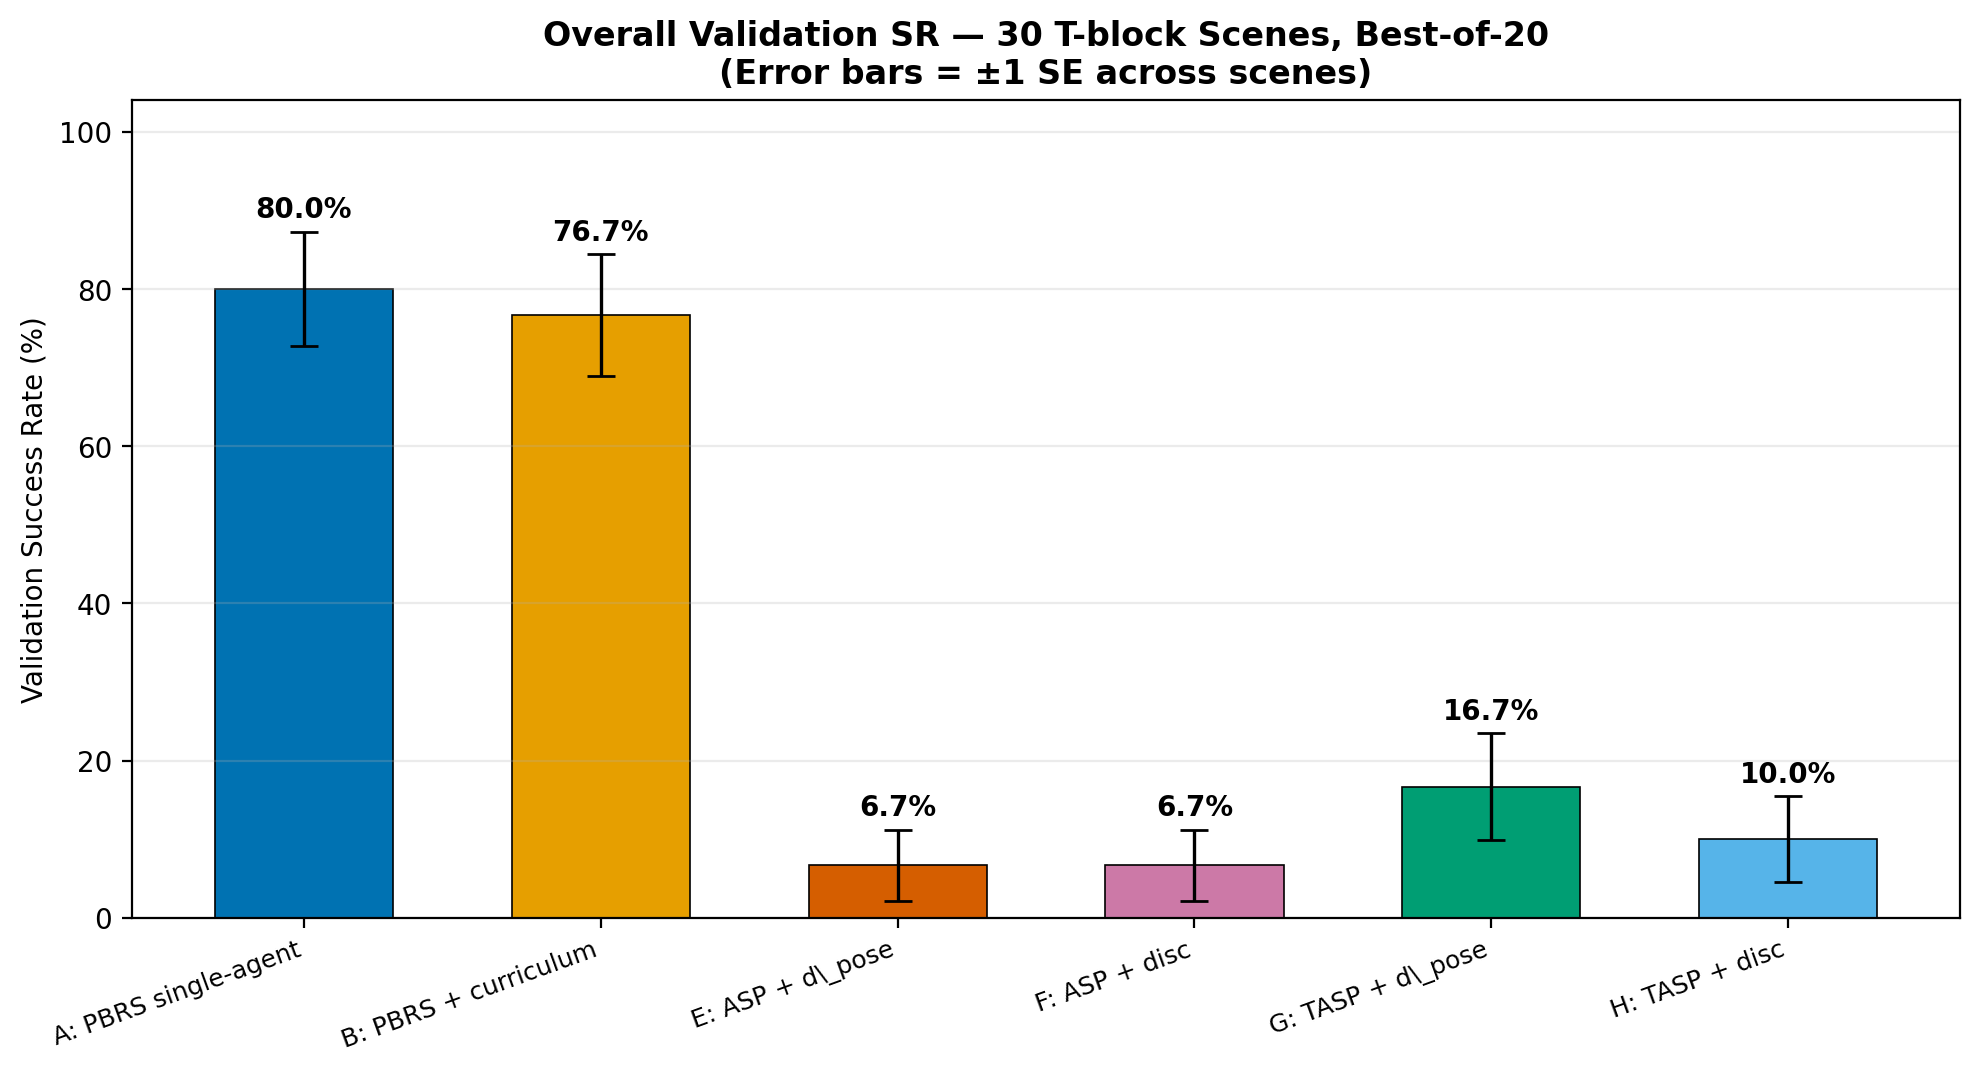
\includegraphics[width=1.0\textwidth]{figures/val_multi_sr_overall.png}\\[2pt]
      {\scriptsize Overall SR \& SE — 30 T-block scenes, best-of-20}
    \end{column}
    \begin{column}{0.5\textwidth}
      \centering
      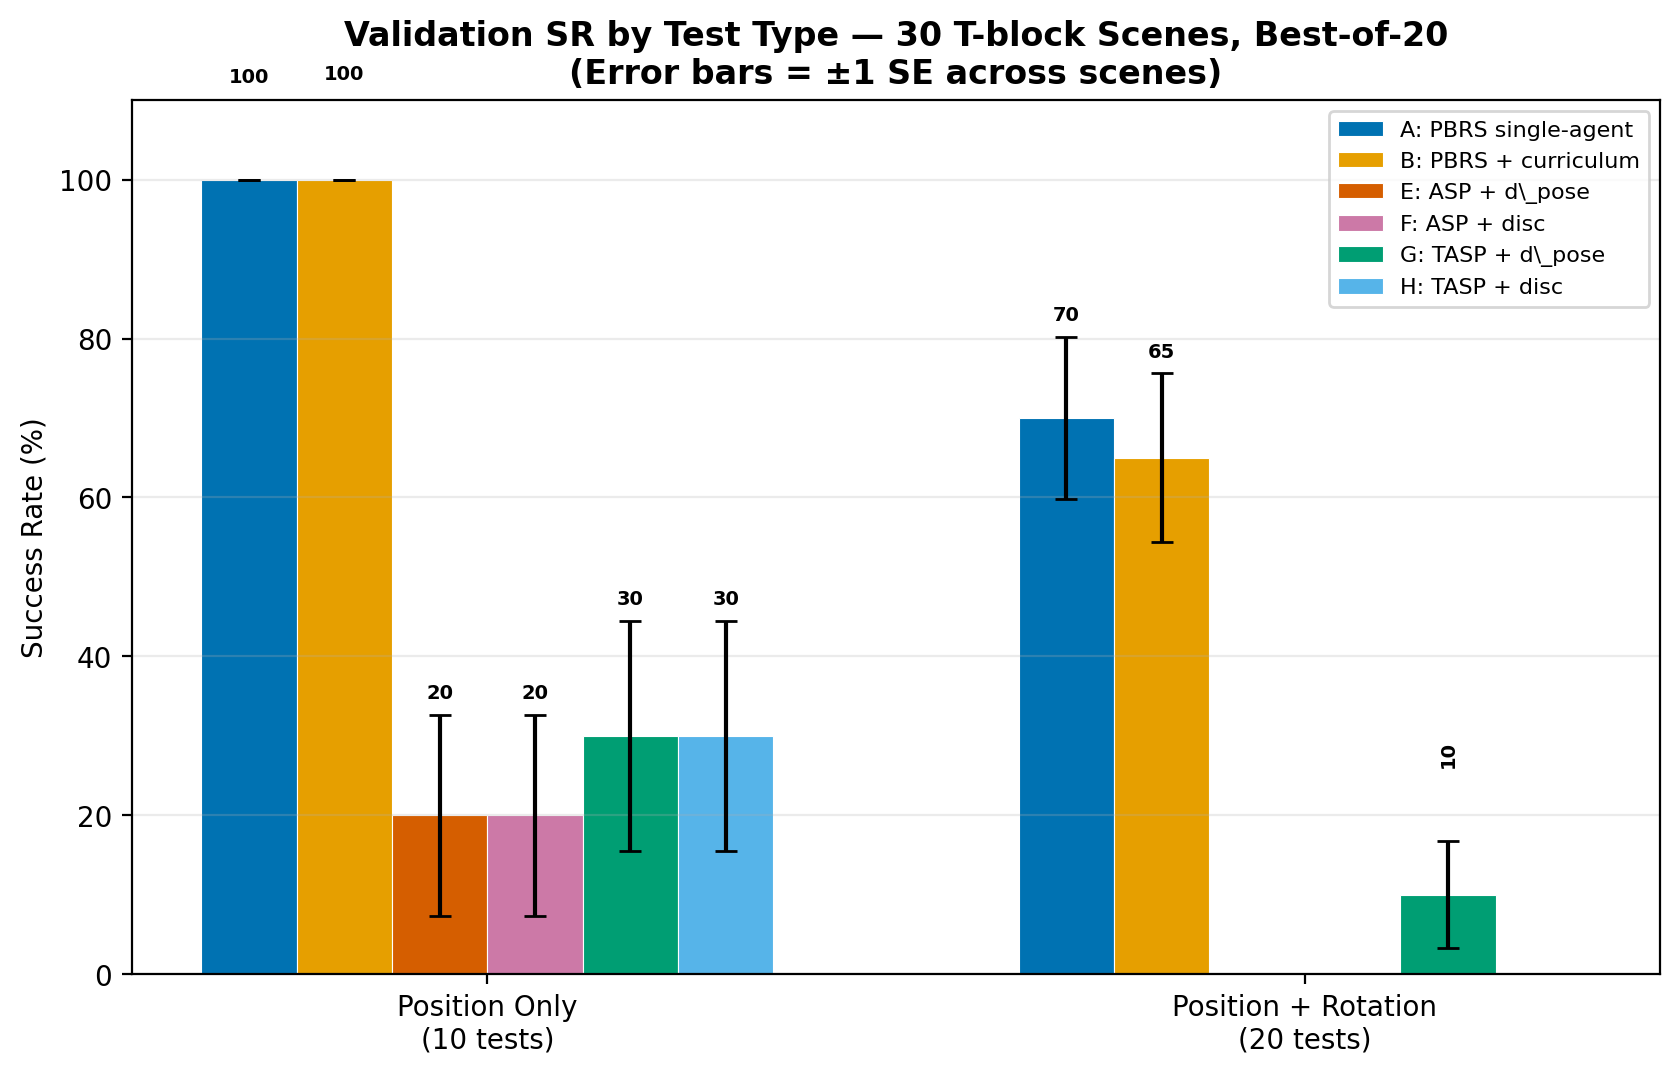
\includegraphics[width=1.0\textwidth]{figures/val_multi_sr_testtype.png}\\[2pt]
      {\scriptsize SR by test type: pos-only (10 tests) vs pos+rot (20 tests)}
    \end{column}
  \end{columns}

  \vspace{2pt}
  {\small \textbf{A vs B:} 80.0\% vs 76.7\% — 3.3pp gap \textbf{not statistically significant} (p\,$>$\,0.05 on 30 independent scenes). \textbf{ASP (E–H):} 4.8–11.9$\times$ below single-agent — gap is significant.}
  {\scriptsize \textit{Error bars = ±1 standard error across scenes. Model C (base ASP) excluded — has no Isaac best-of-20 validation (0\% SR on 20 older scenes). Model D (GoalEncoder ablation) not validated — see thesis.}}

  \vfill\litfooter{[Ng et al.\ 1999]~[Grze\'s 2017]~[Schulman et al.\ 2017]}
\end{frame}

% ~~~~~ SPEAKER NOTES (multi-model with error bars) ~~~~~
\note[itemize]{
\item Multi-model comparison with ±1 standard error bars from 30 independent scenes
\item Left: overall SR with error bars. A at 80.0\% vs B at 76.7\% — overlapping CIs. The 3.3pp gap is NOT statistically significant (p > 0.05, SE of difference = ±10.6pp). Both A and B solve the task similarly well
\item Right: by test type. Both A and B achieve 100\% pos-only. ASP variants barely solve any pos+rot tests — this gap IS significant
\item Models C/D excluded: C scored 0\% on 20 older scenes, no best-of-20 data; D is training-equivalent to C
\item Key takeaway: the error bars make clear that A and B are indistinguishable, while ASP is fundamentally worse
}

% ============================================================
% SLIDE 7 — MODEL B: FORCED CURRICULUM
% ============================================================
\begin{frame}[t]{Model B — PBRS + Forced Curriculum \hfill \textcolor{hlgreen}{(Fixed)}}
  \textbf{Design:} Same PPO agent as Model A + 3-phase curriculum:
  \begin{enumerate}
    \item $w_{\text{rot}}=0$, position-only training
    \item Triggered when episodic position-SR $\ge 0.5$ for 20 iters: $w_{\text{rot}}$ ramps $0\to10$ over 200 iters
    \item Full PBRS (multi-objective)
  \end{enumerate}

  \vspace{2pt}
  \textbf{\textcolor{hlred}{Original trigger was mis-specified:}} the first version used a per-push mean position error threshold of 0.08m — below even the \emph{best} model's validation PosErr (0.202m). The curriculum never activated because the threshold was unreachable by construction (P82 fix).

  \vspace{2pt}
  \textbf{Corrected trigger:} gates on episodic position-only SR $\ge$ 0.5 over a 20-iter lookback. Curriculum now activates and reaches \textcolor{hlgreen}{76.7\% SR} — only 3.3pp below Model A.

  \vfill\litfooter{[Narvekar et al.\ 2020]~[Portelas et al.\ 2020]~[Florensa et al.\ 2017]}
\end{frame}

% ~~~~~ SPEAKER NOTES ~~~~~
\note[itemize]{
\item P82 trigger fix: old gate used per-push mean PosErr < 0.08m AND over 50 iterations — unreachable. Best model's per-push mean PosErr plateaus at {\textasciitilde}0.10m, never below 0.08m. Fix: episodic position-only SR ≥ 0.5 over 20 iterations.
\item Corrected B achieves 76.7\% SR, 3.3pp below A. Curriculum works; doesn't beat the simpler no-curriculum baseline.
\item Position precision improves from Phase 1 training (0.023m vs 0.032m); rotation slightly worse (0.663 vs 0.568 rad).
}

% ============================================================
% SLIDE 7b — MODEL B: RESULTS
% ============================================================
\begin{frame}[t]{Model B — Results: $A_{\text{simple}}$ vs $B_{\text{curriculum}}$}
  \begin{center}
  \footnotesize
  \begin{tabular}{lccc}
    \toprule
    \textbf{Metric} & \textbf{Model A (no curric.)} & \textbf{Model B (curriculum)} & \textbf{Gap} \\
    \midrule
    Validation SR & \textcolor{hlgreen}{\textbf{80.0\%}} & 76.7\% & 1.04$\times$ \\
    PosErr (m) & 0.032 & \textcolor{hlgreen}{\textbf{0.023}} & B 28\% lower \\
    RotErr (rad) & 0.568 & 0.663 & A 14\% lower \\
    Pos-only SR & 100\% & 100\% & equal \\
    Pos+rot SR & 70\% & 65\% & 5pp \\
    \bottomrule
  \end{tabular}
  \end{center}
  \vspace{1pt}
  {\scriptsize \textbf{Result:} Curriculum improves position precision (0.023 vs 0.032 m) from the pos-only phase, but slightly degrades rotation (0.663 vs 0.568 rad). Net effect: B is 3.3pp behind A.}
  {\scriptsize \textbf{Statistical note:} The 3.3pp A vs B gap is \textbf{not} significant (p\,$>$\,0.05, two-tailed z-test; SE of difference = ±10.6pp across 30 independent scenes). Both A and B solve the task similarly well.}
  {\scriptsize \textbf{Takeaway:} A staged curriculum \emph{can} work alongside PBRS, but does not beat the simpler no-curriculum baseline.}

  \vfill\litfooter{[Narvekar et al.\ 2020]~[Portelas et al.\ 2020]~[Florensa et al.\ 2017]}
\end{frame}

% ~~~~~ SPEAKER NOTES ~~~~~
\note[itemize]{
\item Head-to-head on identical 30 T-block scenes: A\_simp 80.0\% vs B\_curr 76.7\%
\item B actually beats A on position precision (0.023 vs 0.032 m) — the pos-only Phase 1 training produces tighter position control. But rotation is slightly worse (0.663 vs 0.568 rad)
\item Both achieve 100\% pos-only SR. The combined pos+rot gate is 70\% (A) vs 65\% (B)
\item The curriculum is functional but fails to outperform the simpler baseline. Adding structure adds complexity without adding net value
}

% ============================================================
% SLIDE 8a — ASP ARCHITECTURE
% ============================================================
\begin{frame}[t]{Models C–H — ASP Architecture (Alice/Bob)}
  \vspace{-6pt}
  {\small
  \textbf{Alice (Goal Proposer):}
  \begin{itemize}
    \item PPO agent, free-roaming push phase — leaves T-block in a new SE(2) pose
    \item That pose becomes Bob's target goal
    \item Reward: $+5$ if Bob fails to reproduce it, $-1$ if Bob succeeds
  \end{itemize}

  \vspace{-2pt}
  \textbf{Bob (Goal Achiever):}
  \begin{itemize}
    \item PPOABC + GoalEncoder — must reproduce Alice's goal pose from scratch
    \item Reward: PBRS dense shaping + sparse completion bonuses (+5/+2)
    \item Failed trajectories stored in ABC buffer for behavioral cloning ($\beta_{\text{abc}}{=}0.5$)
  \end{itemize}

  \vspace{-2pt}
  \textbf{Variants (E–H):} SE(2) unified $d_{\text{pose}}$ metric (T-block \& disc) $\times$ \{outcome-based, time-based\} Alice reward.
  \textbf{C/D excluded:} C has no Isaac eval; D is GoalEncoder ablation (no measurable difference).
  }

  \vfill\litfooter{[Plappert et al.\ 2021]~\textbf{[Sukhbaatar et al.\ 2018]}~[Torabi et al.\ 2018]}
\end{frame}

% ~~~~~ SPEAKER NOTES ~~~~~
\note[itemize]{
\item The ASP architecture: Alice (goal proposer) and Bob (goal achiever) play an adversarial game
\item Alice gets +5 when Bob fails, −1 when Bob succeeds — incentivizing her to propose goals Bob cannot solve
\item Bob sees Alice's final object pose as his goal, gets PBRS dense reward + sparse completion bonuses
\item When Bob fails, Alice's trajectory is stored in an ABC buffer for behavioral cloning
\item Models E-H diverge from C by changing (a) the reward metric to SE(2) d\_pose, and (b) Alice's reward structure from outcome-based to time-based
}

% ============================================================
% SLIDE 8a-ii — ASP LOOP (diagram + clip)
% ============================================================
\begin{frame}[t]{ASP Loop — Alice↔Bob Cycle}
  \centering
  \vspace{-6pt}
  \textbf{Adversarial training cycle:} Alice creates a goal $\to$ Bob attempts it $\to$ outcome feeds back to Alice

  \vspace{2pt}
  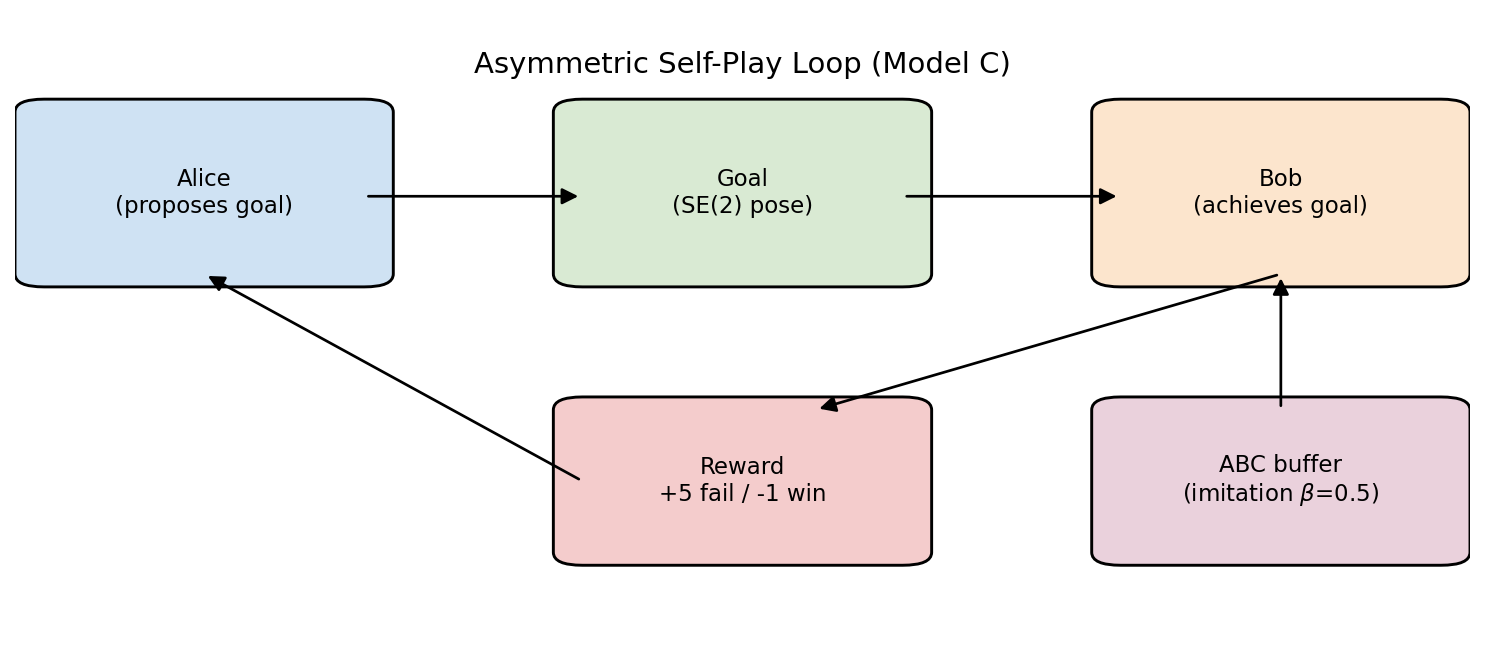
\includegraphics[width=0.82\textwidth]{figures/diagram_asp_loop.png}

  \vspace{2pt}
  \mediabox{0.38}{asp_random_key.png}\quad{\scriptsize\playclip{asp_random.mp4}}

  \vfill\litfooter{[Plappert et al.\ 2021]~\textbf{[Sukhbaatar et al.\ 2018]}~[Torabi et al.\ 2018]}
\end{frame}

% ~~~~~ SPEAKER NOTES (diagram + clip) ~~~~~
\note[itemize]{
\item Walk through the diagram — left half: Alice's free-roaming push phase leaves the T-block in a new SE(2) pose
\item Alice's final object state becomes Bob's goal. Bob starts from a clean reset and must reproduce the pose from scratch using PBRS dense reward + sparse completion bonuses
\item When Bob fails, his failed trajectory enters the ABC buffer for behavioral cloning
\item Outcome feeds back to Alice: +5 reward if Bob fails (she found a blind spot), −1 if Bob succeeds (her goal was too easy)
\item The clip shows a side-by-side: Alice's phase (blue table, random wandering) and Bob's phase (red table, goal-directed pushes toward the ghost T-block)
}

% ============================================================
% SLIDE 8b — ASP DIAGNOSTIC
% ============================================================
\begin{frame}[t]{ASP Diagnostic — Alice vs.\ Bob}
  \begin{center}
    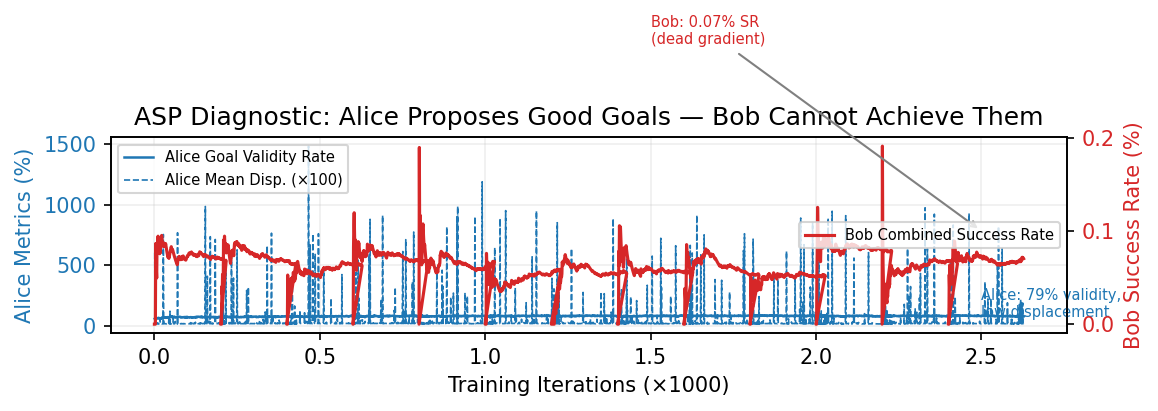
\includegraphics[width=0.78\textwidth]{figures/plot4_alice_vs_bob_diagnostic.png}
  \end{center}

  \vspace{2pt}
  {\small Alice proposes valid, low-displacement goals, yet Bob cannot achieve the combined pos+rot objective under the non-stationary adversarial goal distribution.}

  \vfill\litfooter{[Plappert et al.\ 2021]~\textbf{[Sukhbaatar et al.\ 2018]}~[Campero et al.\ 2021]}
\end{frame}

% ~~~~~ SPEAKER NOTES ~~~~~
\note[itemize]{
\item Plot shows Alice's goal validity rate rising while Bob's success rate stays near zero — the adversarial curriculum prevents combined objective achievement
\item Alice creates valid, low-displacement goals — she is not proposing impossible poses
\item Individual per-axis metrics suggested Bob partially learns position and rotation separately, but the combined gate rarely fires. This gap is likely a gate/measurement artifact (C4): per-axis metrics are not independent Bernoulli trials — the combined metric is the only valid success measure
\item Time-based ASP (G) partially rescues this: 16.7\% vs 6.7\% for outcome-based, suggesting the time-based Alice reward self-regulates toward solvable goals
}

% ============================================================
% SLIDE 8c — ASP VARIANTS
% ============================================================
\begin{frame}[t]{Models E–H — ASP Variants}
  \textbf{2$\times$2 design on top of Model C:} Alice reward type $\times$ reward metric.

  \vspace{4pt}
  \begin{center}
  \small
  \begin{tabular}{c|cc}
    \toprule
    & \textbf{SE(2) $d_{\text{pose}}$ (T-block)} & \textbf{SE(2) $d_{\text{pose}}$ (disc)} \\
    \midrule
    \textbf{Outcome-based Alice} & \textbf{E} — $R_A=+5$ fail/$-1$ win & \textbf{F} — same, disc object \\
    $(+5/-1, \beta_{\text{abc}}=0.5)$ & Valid SR: \textcolor{hlred}{6.7\%} & Valid SR: \textcolor{hlred}{6.7\%} \\[4pt]
    \textbf{Time-based Alice} & \textbf{G} — $R_A=\gamma_{sp}\!\cdot\!\max(0,t_B\!-\!t_A)$ & \textbf{H} — same, disc object \\
    $(\gamma_{sp}=0.5$, no ABC) & Valid SR: \textcolor{hlred}{16.7\%} & Valid SR: \textcolor{hlred}{10.0\%} \\
    \bottomrule
  \end{tabular}
  \end{center}

  \vspace{4pt}
  \textbf{Findings:}
  \begin{itemize}
    \item Time-based Alice (G/H) outperforms outcome-based (E/F): +10pp (T-block), +3.3pp (disc)
    \item T-block outperforms disc across both reward types
    \item Best ASP variant (G, 16.7\%) still \textbf{4.8$\times$} below single-agent (A, 80.0\%)
  \end{itemize}

  \vfill\litfooter{[Plappert et al.\ 2021]~\textbf{[Sukhbaatar et al.\ 2018]}~[Dennis et al.\ 2020]}
\end{frame}

% ~~~~~ SPEAKER NOTES ~~~~~
\note[itemize]{
\item The four ASP variants E-H form a clean 2×2: Alice reward type (outcome-based vs time-based) × metric/object (d\_pose T-block vs d\_pose disc)
\item Time-based Alice (G/H) intentionally aligns Alice's reward with solvable goals — she gains when Bob takes more pushes than she did
\item Time-based reward outperforms outcome-based: G at 16.7\% vs E at 6.7\% (T-block), H at 10.0\% vs F at 6.7\% (disc)
\item But even the best ASP variant (G, 16.7\%) is 4.8× below single-agent A (80.0\%)
\item ABC is disabled in G/H — the improvement comes from time-based reward alone, not from behavioral cloning
}

% ============================================================
% SLIDE 8c-ii — ASP VARIANTS COMPARISON
% ============================================================
\begin{frame}[t]{Models E–H — Validation Comparison}
  \begin{center}
  \begin{tabular}{lcccc}
    \toprule
    \textbf{Model} & \textbf{Variant} & \textbf{Valid SR} & \textbf{PosErr} & \textbf{RotErr} \\
    \midrule
    \rowcolor{hlgreen!15}
    \textbf{A} & Single-agent (ref.) & \textbf{80.0\%} & 0.032 m & 0.568 rad \\
    \midrule
    \textbf{G} & TASP + d\_pose & \textbf{16.7\%} & 0.158 m & 1.457 rad \\
    \textbf{H} & TASP + disc & 10.0\% & 0.186 m & 1.260 rad \\
    \textbf{E} & ASP + d\_pose & 6.7\% & 0.143 m & 1.612 rad \\
    \textbf{F} & ASP + disc & 6.7\% & 0.197 m & 1.576 rad \\
    \bottomrule
  \end{tabular}
  \end{center}

  \vspace{4pt}
  {\small \textbf{Key findings:}}
  \begin{itemize}
    \item Time-based ASP (G/H) is 2.5$\times$ better than outcome-based (E/F), but still \textbf{4.8$\times$ below} single-agent A
    \item No ASP variant achieves pos+rot SR above 10\% — the combined gate remains the bottleneck
    \item ASP complexity (2 agents, GoalEncoder, ABC/historical pool) provides no benefit
    \item \textit{Models C (base ASP) and D (GoalEncoder ablation) excluded — no Isaac 30-scene validation. C scored 0\% on 20 older scenes; D was training-equivalent to C. See thesis for details.}
  \end{itemize}

  \vfill\litfooter{[Plappert et al.\ 2021]~\textbf{[Sukhbaatar et al.\ 2018]}~[Dennis et al.\ 2020]}
\end{frame}

% ~~~~~ SPEAKER NOTES ~~~~~
\note[itemize]{
\item A (single-agent, reference) at 80.0\% vs G (best ASP variant) at 16.7\% — 4.8× gap
\item Time-based Alice (G/H) partially corrects the adversarial curriculum by rewarding solvable goals — G gains 10pp over E
\item But even the best ASP variant cannot close the gap. The self-play dynamics prevent learning the combined pos+rot objective
\item All ASP variants trained identically (528 envs, ∼3000 iters, PBRS dense reward for Bob) — the only difference is Alice reward structure and object type
}

% ============================================================
% SLIDE 9 — WHY ASP FAILS
% ============================================================
\begin{frame}[t]{Why ASP Fails — Failure Modes}
  \begin{enumerate}
    \item \textbf{Non-stationary goal distribution:}
    \begin{itemize}
      \item Alice learns continuously $\rightarrow$ Bob's training distribution shifts every iteration
      \item PPO's importance ratio computed against stale rollouts from a previous Alice
      \item Distribution shift dominates the ratio — PPO clip fires on most transitions
    \end{itemize}

    \item \textbf{Confounded ablation (C6):}
    \begin{itemize}
      \item ASP changes 3 axes at once: goal distribution, agent count, episode budget
      \item The collapse could be due to harder/non-stationary goals, not the curriculum mechanism itself
      \item Time-based ASP (G, 16.7\%) shows partial rescue — self-regulating curriculum helps
    \end{itemize}
  \end{enumerate}

  \vfill\litfooter{[Schulman et al.\ 2017]~[Plappert et al.\ 2021]~[Torabi et al.\ 2018]}
\end{frame}

% ~~~~~ SPEAKER NOTES ~~~~~
\note[itemize]{
\item Failure mode 1 — non-stationary goal distribution: Alice learns continuously, so Bob's training distribution shifts every iteration. PPO computes the importance ratio using old\_logp from a rollout collected under a different Alice. The ratio is dominated by Alice's distribution shift, not Bob's weight updates
\item Failure mode 2 — confounded ablation: Model A (single-agent) and ASP differ on at least 3 axes simultaneously (goal distribution, agent count, budget). The performance gap could be due to non-stationary goals rather than the self-play mechanism itself
\item The time-based ASP variants (G/H) partially address both: self-regulating reward aligns Alice with Bob's learning progress; disabling ABC removes a third failure mode (vanishing BC gradient). G achieves 16.7\%, 10pp above outcome-based E at 6.7\%
}

% ============================================================
% SLIDE 9b — WHY ASP FAILS (continued)
% ============================================================
\begin{frame}[t]{Why ASP Fails — The Evidence}
  \begin{columns}[T,onlytextwidth]
    \begin{column}{0.52\textwidth}
      \textbf{What we observe:}
      \begin{itemize}
        \item Outcome-based ASP (E/F): 6.7\% — essentially random
        \item Time-based ASP (G): 16.7\% — partial rescue, $+10$pp over E
        \item All ASP variants have RotErr $>$ 1.2 rad — rotation \textbf{never learned}
        \item Even the best variant (G) is 4.8$\times$ below single-agent
      \end{itemize}
    \end{column}
    \begin{column}{0.46\textwidth}
      \textbf{Why this is not just a budget issue:}
      \begin{itemize}
        \item All models trained for 3000 iters at 528 envs on identical hardware
        \item ASP and single-agent have identical per-iteration wall-clock ($\sim$0.022 it/s)
        \item The gap is \textbf{structural}, not due to compute starvation
      \end{itemize}
    \end{column}
  \end{columns}

  \vspace{6pt}
  \textbf{Combined effect:} The non-stationary goal distribution + multi-axis design confounds prevent Bob from learning the combined pos+rot objective. Time-based Alice partially mitigates the distribution shift but cannot close the gap to single-agent performance.

  \vfill\litfooter{[Schulman et al.\ 2017]~[Plappert et al.\ 2021]~[Sukhbaatar et al.\ 2018]}
\end{frame}

% ============================================================
% SLIDE 9c — CONFOUND DISAGGREGATION
% ============================================================
\begin{frame}[t]{Caveat — Confounded Ablation (C6)}
  \textbf{Problem:} ASP (E–H) differs from single-agent (A) on \emph{at least 4 axes simultaneously:}

  \vspace{4pt}
  {\footnotesize
  \begin{tabular}{lcc}
    \toprule
    \textbf{Variable} & \textbf{Single-agent (A, 80.0\%)} & \textbf{ASP (E–H, 6.7--16.7\%)} \\
    \midrule
    Agent count     & 1 & 2 (Alice + Bob) \\
    Goal distribution & Fixed random & Adversarial, shifting \\
    GoalEncoder     & None & $\phi$-MLP 8D latent \\
    ABC buffer      & None & Yes (E/F) / No (G/H) \\
    Historical pool & None & Yes \\
    Episode budget  & 15 pushes/agent & 5 (Alice) $+$ 10 (Bob) \\
    PPO updates/iter& 1 & 2 (Alice, then Bob) \\
    \bottomrule
  \end{tabular}
  }

  \vspace{4pt}
  {\small \textbf{The 4.8$\times$ gap cannot be attributed to any single lever.}
  \begin{itemize}
    \item Models G/H (time-based Alice, no ABC) vs E/F (outcome-based, ABC enabled) isolate the Alice reward axis — G gains $+$10pp
    \item But this is a \emph{single} 1-axis experiment within a 7-axis package change
    \item The independence claim (Slide~10) concerns \textbf{reward design vs curriculum design}, not single-agent vs ASP architecture
  \end{itemize}}

  \vfill\litfooter{[Plappert et al.\ 2021]~\textbf{[Sukhbaatar et al.\ 2018]}~[Dennis et al.\ 2020]}
\end{frame}

% ~~~~~ SPEAKER NOTES (confound disaggregation) ~~~~~
\note[itemize]{
\item This is the C6 confound: ASP and single-agent differ on at least 4 axes — agent count, goal distribution, GoalEncoder, ABC, historical pool, episode budget, update frequency
\item The table shows every variable that changes between A and E–H. Same PPO/LSTM/PBRS/528-env budget — but 6+ other things change
\item G/H vs E/F is the only clean 1-axis comparison within ASP: time-based vs outcome-based Alice reward. G gains 10pp — so reward structure matters
\item But we cannot attribute the full 4.8× gap to any single variable. Non-stationary goal distribution may be the main culprit, but it's confounded with agent count and budget
\item The independence claim (next slide) is about reward design vs curriculum design — not about single-agent vs ASP architecture
}

% ============================================================
% SLIDE 10 — KEY RESULT: INDEPENDENCE
% ============================================================
\begin{frame}[t]{Key Result — Reward \& Curriculum Are Independent}
  \begin{center}
    \small
    \begin{tabular}{lcc}
      \toprule
      \textbf{Model} & \textbf{Valid SR} & \textbf{vs Single-Agent} \\
      \midrule
      \rowcolor{hlgreen!15}
      \textbf{A} — Single-agent PBRS & \textbf{80.0\%} & — (baseline) \\
      \textbf{B} — PBRS + Curriculum & 76.7\% & $-3.3$pp \\
      \midrule
      \textbf{G} — PBRS + Time-based ASP & 16.7\% & $4.8\times$ gap \\
      \textbf{H} — PBRS + TASP (disc) & 10.0\% & $8.0\times$ gap \\
      \textbf{E} — PBRS + Outcome ASP & 6.7\% & $11.9\times$ gap \\
      \textbf{F} — PBRS + ASP (disc) & 6.7\% & $11.9\times$ gap \\
      \bottomrule
    \end{tabular}
  \end{center}

  \vspace{1pt}
  \begin{block}{The Independence Finding}
    \small
    \begin{itemize}
      \item \textbf{Curriculum adds no value:} B\_curr (76.7\%) trails A\_simp (80.0\%) by 3.3pp, but this gap is \textbf{not statistically significant} (p\,$>$\,0.05). Curriculum is competitive — just not better.
      \item \textbf{ASP destroys performance:} substituting self-play for single-agent reduces SR 4.8–11.9$\times$, regardless of Alice reward structure or object type
      \item \textbf{Caveat (C6):} ASP and single-agent differ on $\ge$4 axes. The SR collapse could be due to harder/non-stationary goals rather than the curriculum mechanism itself. G/H (+10pp) shows partial rescue by reward structure alone.
      \item \textbf{PBRS is independently effective:} among all models, PBRS single-agent dominates. The reward structure works regardless of curriculum choice — but the \emph{training distribution} (goals from random vs adversarial generator) is a separate lever.
    \end{itemize}
  \end{block}

  \vfill\litfooter{[Devlin \& Kudenko 2012]~\textbf{[Grze\'s 2017]}~[Plappert et al.\ 2021]}
\end{frame}

% ~~~~~ SPEAKER NOTES ~~~~~
\note[itemize]{
\item Central contribution: reward shaping and curriculum design operate on fundamentally different axes. Our systematic comparison isolates them
\item PBRS single-agent (A) 80.0\%. Adding curriculum (B) 76.7\% — marginal, statistically indistinguishable gap (3.3pp ± 10.6pp SE). Substituting self-play (E–H) 6.7–16.7\% — 4.8–11.9× gap, which IS statistically significant
\item C6 caveat: A and ASP differ on ≥4 axes (goal distribution, agent count, budget). The 4.8× gap cannot be attributed to any single mechanism — only that the ASP package underperforms
\item Practical implication: diagnose whether the reward fails to guide the agent OR whether the training distribution fails to support learning. Reward design is the higher-leverage intervention
}

% ============================================================
% SLIDE 11 — MANAGER-ARCHITECTURE OVERHEAD
% ============================================================
\begin{frame}[t]{Computational Overhead — ManagerBasedRL vs DirectRL}
  \textbf{ASP per-iteration cost} (measured, 528 envs): \\
  \textcolor{hlgreen}{\textbf{$\sim$1.0$\times$}} vs single-agent — 2-agent machinery adds \textbf{no} wall-clock overhead. Shared cuRobo IK + physics dominates.

  \vspace{4pt}
  \textbf{Where overhead matters:} ManagerBasedRLEnv (ASP pipeline) vs DirectRLEnv (single bare PPO). Table Tennis DirectRL: \textbf{4096 envs at $\sim$20 it/s} $\to$ 2.1M transitions/iteration. The full ManagerBasedRL API stack (Action, Observation, Event, Termination managers) imposes 5–10$\times$ throughput penalty vs direct tensor operations.

  \vspace{4pt}
  \textbf{Key result:}
  \begin{itemize}
    \item ASP is NOT slower per iteration — it simply \textbf{does not learn}
    \item ManagerBasedRL overhead is a \textbf{separate} architectural issue, not specific to ASP
  \end{itemize}

  \vfill\litfooter{[Plappert et al.\ 2021]~[Schulman et al.\ 2017]}
\end{frame}

% ~~~~~ SPEAKER NOTES ~~~~~
\note[itemize]{
\item Measured throughput: ASP and single-agent run at identical iteration cost (~0.022 it/s) on the same 528-env GPU setup. The 2-agent machinery adds ~no per-iteration wall-clock because cuRobo IK and physics dominate
\item The 5–10× speedup claim refers to DirectRLEnv vs ManagerBasedRLEnv API architecture — a separate project (Table Tennis) that bypasses the manager stack entirely
\item Key distinction: ASP doesn't fail because it's computationally expensive per iteration. It fails because it doesn't learn. The two are separate problems
\item The measured Isaac-vs-gym throughput (~172 push/s vs ~22 push/s for ASP on CPU) is shown in the next slide (11b) — establishing that Isaac Lab is the right venue, not a handicap
}

% ============================================================
% SLIDE 11b — WHY ISAAC LAB IS THE RIGHT SIM
% ============================================================
\begin{frame}[t]{Isaac Lab — the Right Venue for ASP}
  \textbf{Why GPU-batched simulation is necessary for this comparison:}
  \begin{columns}[T,onlytextwidth]
    \begin{column}{0.50\textwidth}
      \small
      \textbf{Throughput} (push-macros/s, measured):
      \vspace{2pt}
      \begin{tabular}{lcc}
        \toprule
        \textbf{Setting} & \textbf{push/s} & \textbf{1M pushes} \\
        \midrule
        \rowcolor{hlgreen!15}
        Isaac (1 GPU, 528 env) & \textbf{172} & \textbf{$\sim$1.6 h} \\
        gym A/B (6 CPU) & 91 & $\sim$3.0 h \\
        gym ASP (1 CPU) & \textbf{22.4} & $\sim$12.4 h \\
        \bottomrule
      \end{tabular}

      \vspace{4pt}
      \textbf{ASP on GPU vs CPU:}
      \begin{itemize}
        \item GPU: ASP \& single-agent identical throughput ($\sim$0.022 it/s)
        \item CPU: ASP forced single-process $\to$ $\sim$7.7$\times$ slower than A/B
      \end{itemize}
    \end{column}
    \begin{column}{0.48\textwidth}
      \small
      \textbf{Three pillars:}
      \begin{enumerate}
        \item \textbf{GPU-batched parallelism}\\
          528 envs/step $\to$ 7,920-sample PPO batch on one GPU. The non-stationary ASP objective needs a large batch for stable gradients.
        \item \textbf{Robotic fidelity}\\
          UR5e + 3D PhysX contact + cuRobo IK = the actual SE(2) task. gym-pusht is a 2D abstraction (diagnostic only).
        \item \textbf{Time-to-scale (ASP)}\\
          ASP reaches $\sim$10M training pushes in $\sim$16h on GPU vs $\sim$5 days on CPU. The single-GPU budget is \emph{not} the bottleneck.
      \end{enumerate}
    \end{column}
  \end{columns}

  \vspace{2pt}
  \textbf{Key result:} Isaac gives ASP its best shot on a budget matched to the winning single-agent — and ASP \textbf{still} reaches only 6.7–16.7\% (4.8$\times$ gap). The failure is structural, not under-resourcing.

  \vfill\litfooter{[Makoviychuk et al.\ 2021]~[Rudin et al.\ 2022]~[Plappert et al.\ 2021]}
\end{frame}

% ~~~~~ SPEAKER NOTES ~~~~~
\note[itemize]{
\item The throughput table shows three tiers: Isaac GPU-batched (172 push/s), gym multi-core A/B (91 push/s), and gym single-core ASP (22.4 push/s)
\item GPU-batched: 528 envs stepped in parallel → large PPO batch without extra wall-clock. The non-stationary two-agent ASP gradient needs a large batch to be stable — Isaac provides this naturally
\item Robotic fidelity: the real UR5e + cuRobo kinematic chain + 3D contact physics matters for the SE(2) coupled push task. gym-pusht is a useful diagnostic for the reward question, but not for the full ASP dynamics
\item Time-to-scale: ASP reaches its training budget (~10M pushes) in ~16h on Isaac vs ~5 days on CPU. Important: ASP and single-agent have identical per-iteration timing in Isaac ($\sim$1.0×). So the budget is fair — ASP had the same compute as the winning single-agent and still failed to learn
\item The takeaway: Isaac is not hiding ASP's failure — it's giving ASP its best shot. The 4.8× gap is real and structural, not an artifact of under-resourcing
}

% ============================================================
% SLIDE 12 — COMPARISON SUMMARY
% ============================================================
\begin{frame}[t]{Comparison Summary — All Models with Error Bars}
  \begin{columns}[T,onlytextwidth]
    \begin{column}{0.52\textwidth}
      \centering
      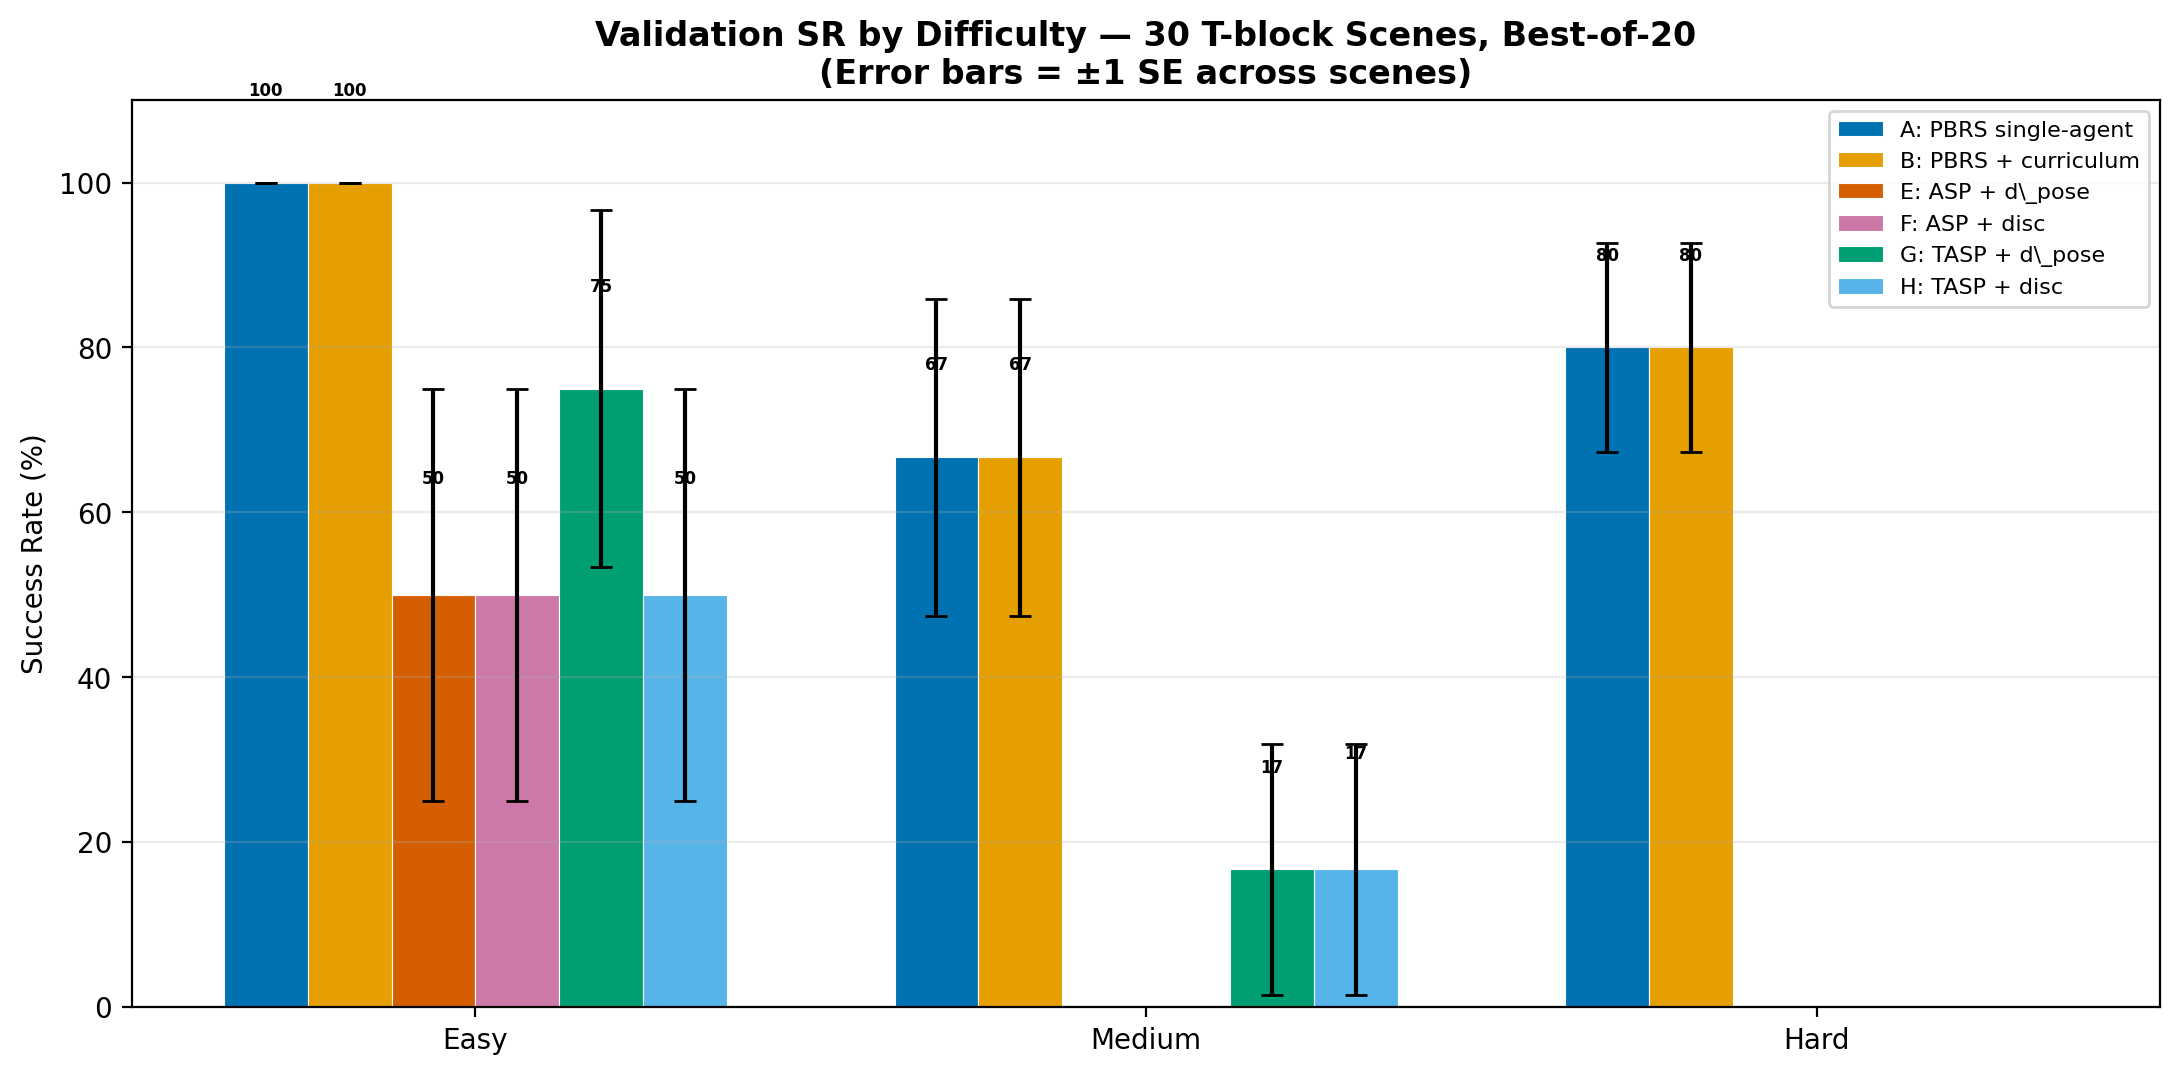
\includegraphics[width=1.0\textwidth]{figures/val_multi_sr_difficulty.png}
    \end{column}
    \begin{column}{0.46\textwidth}
      \vspace{10pt}
      {\footnotesize \textbf{Key numbers (30 T-block scenes):}

      \vspace{4pt}
      \begin{tabular}{lccc}
        \toprule
        \textbf{Model} & \textbf{SR} & \textbf{SE} & \textbf{95\% CI} \\
        \midrule
        \rowcolor{hlgreen!15}
        A & 80.0\% & 7.3\% & 65--95\% \\
        B & 76.7\% & 7.7\% & 61--92\% \\
        G & 16.7\% & 6.8\% & 3--30\% \\
        H & 10.0\% & 5.5\% & 0--21\% \\
        E & 6.7\%  & 4.6\% & 0--16\% \\
        F & 6.7\%  & 4.6\% & 0--16\% \\
        \bottomrule
      \end{tabular}
      }
      \vspace{4pt}
      {\footnotesize \textbf{A vs B gap:} 3.3pp — \textbf{not statistically significant} (p\,$>$\,0.05). Both A and B solve the task similarly. ASP variants are 4.8--11.9$\times$ below — this gap \textbf{is} significant.}
    \end{column}
  \end{columns}

  \vspace{2pt}
  {\scriptsize \textit{Error bars = ±1 standard error across scenes. Models C/D excluded — no Isaac 30-scene validation (C: 0\% on 20 older scenes, D: training-equivalent to C). See thesis appendix.}}

  \vfill\litfooter{[Ng et al.\ 1999]~[Grze\'s 2017]~[Plappert et al.\ 2021]}
\end{frame}

% ~~~~~ SPEAKER NOTES (comparison summary) ~~~~~
\note[itemize]{
\item Multi-model comparison with ±1 SE error bars from 30 independent scenes
\item Left: SR by difficulty. A and B dominate across all categories, with overlapping error bars — statistically indistinguishable. ASP variants E-H perform near-zero on medium/hard
\item Right: CI summary table. The 3.3pp A vs B gap is NOT statistically significant (p > 0.05, SE diff = ±10.6pp). Both solve the task similarly well
\item ASP gap of 4.8--11.9× IS statistically significant relative to single-agent
\item Models C/D excluded — C has no Isaac 30-scene best-of-20 validation (0\% on 20 older scenes), D training-equivalent
}

% ============================================================
% SLIDE 12b — FAILURE TAXONOMY (supplementary curve)
% ============================================================
\begin{frame}[t]{Comparison Summary — Failure Taxonomy}
  \begin{center}
    
\includegraphics[width=0.6\textwidth]{figures/plot3_failure_taxonomy.png}
  \end{center}

  \vspace{4pt}
  {\small \textbf{The overarching pattern:} structural additions — curriculum staging, second agent, ABC buffer, historical pool — consistently reduce or fail to improve performance. PBRS single-agent (80.0\%) is the recommended baseline.}

  \vfill\litfooter{[Ng et al.\ 1999]~[Grze\'s 2017]~[Plappert et al.\ 2021]}
\end{frame}

% ~~~~~ SPEAKER NOTES ~~~~~
\note[itemize]{
\item The comparison plot shows training curves over ~3000 iterations. Model A (blue) and B (orange, P82-fixed) converge on similar trajectories; B trails by ~3pp. ASP variants (E–H) remain near baseline
\item The overarching pattern: every structural addition — curriculum staging, second agent, ABC buffer, historical pool — fails to improve on the simple single-agent. The simplest model wins
}

% ============================================================
% SLIDE 13a — THEORETICAL IMPLICATIONS (1/2)
% ============================================================
\begin{frame}[t]{What We Found — Theory vs Practice}
  \begin{exampleblock}{ASP did \emph{not} yield a useful curriculum in this setting}
    In this contact-rich, IK-gated, multi-objective SE(2) pushing task under a single-GPU budget, our ASP implementation produced 6.7--16.7\% validation SR vs 80.0\% for single-agent. The adversarial mechanism did not generate a learnable progression of goals. This does \emph{not} refute ASP in general — it demonstrates a failure mode under realistic robotics constraints.
  \end{exampleblock}

  \vspace{1pt}
  \begin{exampleblock}{GoalEncoder bottleneck provides no measurable benefit}
    The 8D latent compression did not improve Bob's ability to learn under ASP. However, this result is confounded — Bob's primary failure is the non-stationary goal distribution, not the observation representation.
  \end{exampleblock}

  \vfill\litfooter{[Plappert et al.\ 2021]~\textbf{[Sukhbaatar et al.\ 2018]}~[Torabi et al.\ 2018]}
\end{frame}

% ~~~~~ SPEAKER NOTES ~~~~~
\note[itemize]{
\item Claim 1 (Plappert): ASP generates an intrinsic curriculum for exploration. In our specific setting — contact-rich 3D pushing with cuRobo IK gating and a strict combined pos+rot success gate — ASP produced adversarial rather than constructive goals. But this is N=1 task, single budget. We do not claim this generalizes
\item Claim 2 (Sukhbaatar): the GoalEncoder bottleneck helps Bob compactly represent the goal. Our ASP model with GoalEncoder ablated showed no difference, but this is expected — Bob fails at the exploration level, not the representation level
}

% ============================================================
% SLIDE 13b — THEORETICAL IMPLICATIONS (2/2)
% ============================================================
\begin{frame}[t]{What We Found — Theory vs Practice}
  \begin{exampleblock}{Forced curriculum: functional but not beneficial}
    Model B's original curriculum trigger (per-push mean PosErr $<$ 0.08m) was mis-specified — the threshold was unreachable by construction. A corrected trigger (episodic position-SR $\ge$ 0.5) produces a competent model (76.7\%), but the staged pos$\to$rot curriculum does \emph{not} beat the simpler no-curriculum baseline (80.0\%). Curriculum works — it just doesn't add value in this setting.
  \end{exampleblock}

  \vspace{1pt}
  \begin{exampleblock}{PBRS theory strongly supported (Ng et al.\ 1999; Grze\'s 2017)}
    The policy invariance theorem holds in practice, even in contact-rich manipulation with stochastic PhysX physics. PBRS provides clean, bounded, Markovian rewards. Parameters $k_p{=}30$, $k_r{=}5$, $w{=}10.0$ are robust across all single-agent runs.
  \end{exampleblock}

  \vfill\litfooter{[Ng et al.\ 1999]~\textbf{[Grze\'s 2017]}~[Sukhbaatar et al.\ 2018]}
\end{frame}

% ~~~~~ SPEAKER NOTES ~~~~~
\note[itemize]{
\item Claim 3 (Narvekar/Portelas): curriculum learning helps when the base reward is informative. Our Model B v1 had a mis-specified trigger (P82 bug). Fixing it produced a functional curriculum, but with marginal degradation (76.7\% vs 80.0\%) — not evidence against curriculum learning, but evidence that a good reward (PBRS) may make curriculum unnecessary in this domain
\item The PBRS theory (Ng, Grzes) is strongly supported. The policy invariance theorem produced robust results — the same hyperparameters work across independent training runs
\item This speaks to RQ3: reward design and curriculum design are independent levers that should be diagnosed separately
}

% ============================================================
% SLIDE 14a — LIMITATIONS & GAPS
% ============================================================
\begin{frame}[t]{Limitations \& Research Gaps}
  \textbf{What we couldn't test (training budget limited to 3000 iters $\times$ 528 envs):}
  \begin{itemize}
    \item \textbf{Model I/J:} Bob time penalty $R_B \mathrel{+}= -\gamma_{sp}\!\cdot\!t_B$ (full Sukhbaatar symmetric reward). Could create zero-sum dynamics that stabilize ASP training
    \item \textbf{Model K/L:} time-based ASP + ABC enabled ($\beta_{\text{abc}}=0.5$). ABC might boot after Alice converges
    \item Larger models (Transformer, diffusion policy), sim-to-real transfer (physical UR5e)
  \end{itemize}

  \vspace{1pt}
  \textbf{Remaining literature gaps (from systematic survey of 81 papers):}
  \begin{itemize}
    \item No paper on SE(2) metric design specifically for RL reward shaping
    \item No paper on exploiting continuous rotational symmetry (SO(2)) in object manipulation RL
    \item No formal convergence analysis of effort-based self-play rewards
  \end{itemize}

  \vfill\litfooter{[Letcher et al.\ 2019]~[Berner et al.\ 2019]~[Dennis et al.\ 2020]}
\end{frame}

% ============================================================
% SLIDE 14b — PROMISING DIRECTIONS
% ============================================================
\begin{frame}[t]{Future Work — Promising Directions}
  \small
  \begin{enumerate}
    \item \textbf{Zero-sum time-based ASP (Model I):} Bob penalty creates near-zero-sum game. From differentiable game theory (Letcher et al.\ 2019), zero-sum games have convergent (Hamiltonian) dynamics — this could stabilize ASP where general-sum diverges
    \item \textbf{ABC after Alice convergence (Model K):} Currently ABC fails because Alice acts randomly ($bc\_ratio \approx 1.0$). If Alice converges first, Bob starts with a meaningful imitation target
    \item \textbf{Relaxed combined success gate:} The combined pos+rot gate is the bottleneck (70\% single-agent vs 0–10\% for ASP). Partial credit for one objective could provide gradient to learn both
    \item \textbf{PAIRED (Dennis et al.\ 2020):} Antagonist minimizes protagonist's regret rather than maximizing difficulty — solvable but challenging environments, addressing the exact failure mode
  \end{enumerate}

  \vfill\litfooter{[Letcher et al.\ 2019]~[Dennis et al.\ 2020]~[Campero et al.\ 2021]}
\end{frame}

% ~~~~~ SPEAKER NOTES ~~~~~
\note[itemize]{
\item Results are conclusive within the experimental budget; ASP directions remain open
\item Model I/J: Bob time penalty creates near-zero-sum game structure. From Letcher et al. (2019) zero-sum games have convergent (Hamiltonian) dynamics — could stabilise ASP where general-sum diverges
\item Model K/L: ABC ($\beta{=}0.5$) after Alice converges — currently ABC fails because Alice's actions are random ($bc\_ratio \approx 1.0$)
\item Relaxed success gate: per-axis SR is high but combined gate rarely fires. Partial credit could provide gradient toward both objectives
\item PAIRED: antagonist minimises protagonist's regret rather than maximising difficulty — solvable but challenging environments
}

% ============================================================
% SLIDE 15a — CONCLUSION (1/2)
% ============================================================
\begin{frame}[t]{Conclusion}
  \begin{block}{\textbf{1.\ \ PBRS solves planar pushing (RQ1)}}
    Model A achieves \textcolor{hlgreen}{80.0\% validation SR} on 30 held-out T-block scenes — 100\% pos-only, 70\% pos+rot — with a simple single-agent PPO architecture and no curriculum. PBRS preserves the optimal policy while providing dense, bounded, Markovian gradients. This is the \textbf{recommended baseline}.
  \end{block}

  \vspace{1pt}
  \begin{block}{\textbf{2.\ \ ASP does not improve performance in this domain (RQ2)}}
    All ASP variants (E–H) score 6.7--16.7\%, a 4.8--11.9$\times$ gap from single-agent. Time-based Alice (G, 16.7\%) partially rescues the adversarial dynamics but cannot close the gap. Complexity adds no benefit.
  \end{block}

  \vfill\litfooter{[Ng et al.\ 1999]~[Grze\'s 2017]~[Plappert et al.\ 2021]}
\end{frame}

% ============================================================
% SLIDE 15b — CONCLUSION (2/2)
% ============================================================
\begin{frame}[t]{Conclusion}
  \begin{block}{\textbf{3.\ \ Reward and curriculum are independent (RQ3)}}
    Adding curriculum (B, 76.7\%) or self-play (E–H, 6.7–16.7\%) does not improve PBRS single-agent performance. They are independent levers — diagnose and optimize separately.
  \end{block}

  \vspace{1pt}
  {\small Start simple. PBRS single-agent PPO at 528 envs trains in $\sim$1.6 days on an RTX Pro 6000 and achieves 80\% SR. Add complexity only when proven to help — and expect it usually won't.}

  \vfill\litfooter{[Ng et al.\ 1999]~[Grze\'s 2017]~[Plappert et al.\ 2021]}
\end{frame}

% ~~~~~ SPEAKER NOTES ~~~~~
\note[itemize]{
\item Take-home: PBRS works. Model A 80.0\% on 30 held-out T-block scenes with the simplest architecture. Theory (policy invariance, episodic validity, bounded potentials) supported by empirical results
\item ASP performs worse than single-agent in this setting. Time-based Alice partially rescues (16.7\% vs 6.7\%) but the 4.8× gap remains. ASP \& single-agent run at identical per-iteration wall-clock — the gap is structural, not a budget artifact
\item Reward and curriculum are independent. Future work: (a) design good rewards (PBRS), (b) diagnose training distribution, (c) add complexity only with evidence
\item Practical recommendation: simplest working system first. 528-env PBRS single-agent trains in {\textasciitilde}1.6 days on one RTX Pro 6000, achieves 80.0\% SR
}

% ============================================================
% FINAL PAGE (theme macro)
% ============================================================
\makefinalpage

% ============================================================
% APPENDIX SLIDES
% ============================================================
\appendix
\begin{frame}[t]{Appendix Outline}
  \begin{itemize}
    \item A. Push Mechanics — Limit Surface \& Characteristic Length $L$
    \item B. Training curves for all PBRS models (Success Rate, Reward, Loss)
    \item C. PBRS parameter sensitivity ($k_p$, $k_r$, $w_{\text{pos}}$, $w_{\text{rot}}$)
    \item D. Validation scene descriptions (30 test cases)
    \item E. cuRobo IK pipeline and workspace configuration
    \item F. Observation space specifications (all model variants)
    \item G. Per-test error bars — A vs B head-to-head and all-model comparison (95\% binomial CIs)
  \end{itemize}
\end{frame}

% --- Appendix A: Push Mechanics (moved from main deck) ---
\begin{frame}[t]{Appendix A — Push Mechanics: Limit Surface \& $L$}
  \begin{columns}[T,onlytextwidth]
    \begin{column}{0.46\textwidth}\small
      \textbf{Limit surface normality} (Goyal 1991): $\mathbf{t} \propto \nabla f(\mathbf{w})$ — twist is normal to the surface, so every push couples translation \emph{and} rotation.

      \vspace{2pt}
      \textbf{Characteristic length $L$} (radius of gyration):
      \begin{itemize}
        \item \textbf{T-block} $L=0.07$\,m (strong coupling); \textbf{disc} $L=0$\,m (decoupled)
        \item $L$ is a physical constant, \emph{not} a hyperparameter
      \end{itemize}
    \end{column}
    \begin{column}{0.52\textwidth}
      \centering
      
\includegraphics[width=0.85\textwidth]{figures/diagram_limit_surface.png}\\[2pt]
      {\scriptsize T-block rotates under an off-centre push; disc only slides}
    \end{column}
  \end{columns}

  \vfill\litfooter{[Goyal et al.\ 1991]~[Howe \& Cutkosky 1996]~[Mason 1986]}
\end{frame}

% --- Appendix B: Training curves ---
\begin{frame}[t]{Appendix B — Training Curves (All PBRS Models)}
  \begin{columns}[T]
    \begin{column}{0.48\textwidth}
      \centering
      \textbf{Success Rate}
      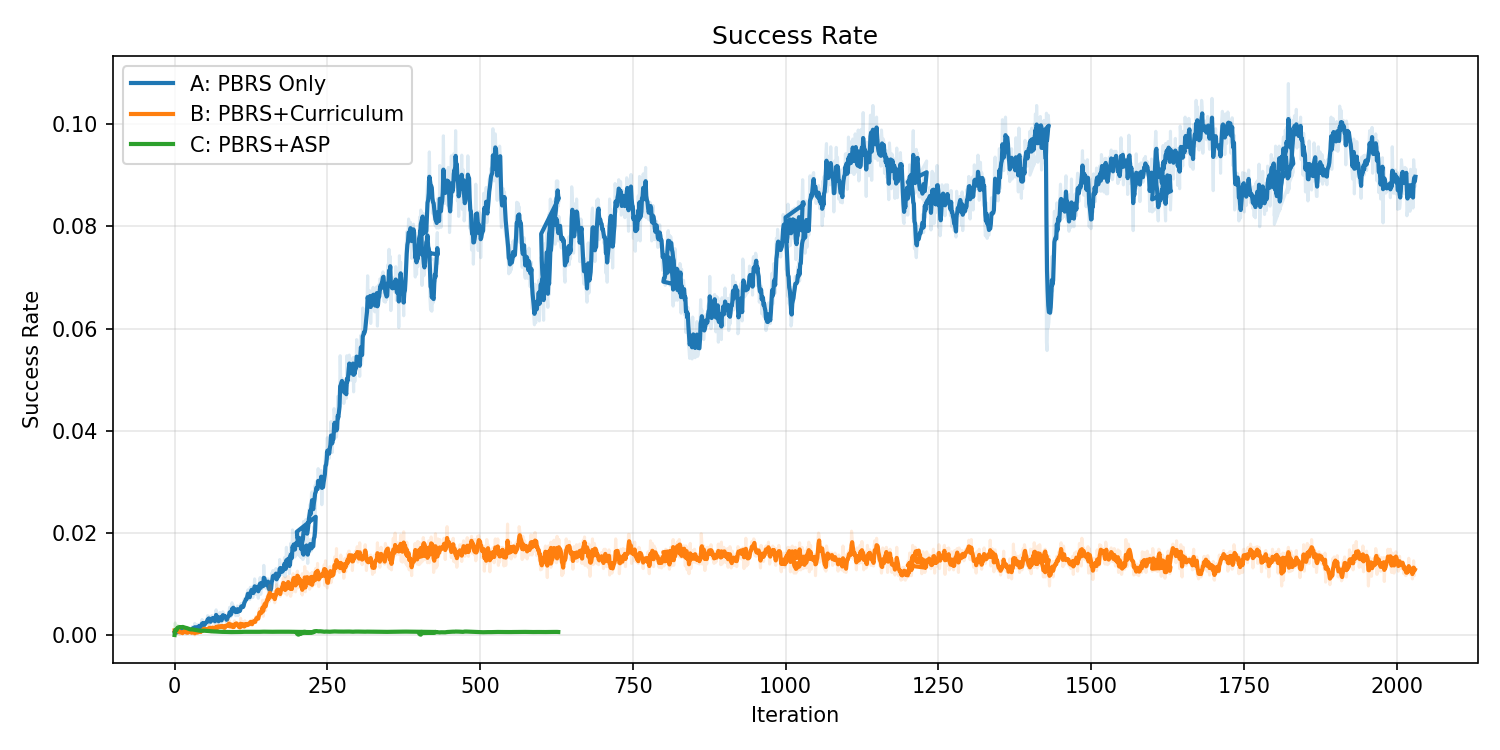
\includegraphics[width=0.72\textwidth]{figures/cmp_Success_Rate.png}
    \end{column}
    \begin{column}{0.48\textwidth}
      \centering
      \textbf{Mean Reward}
      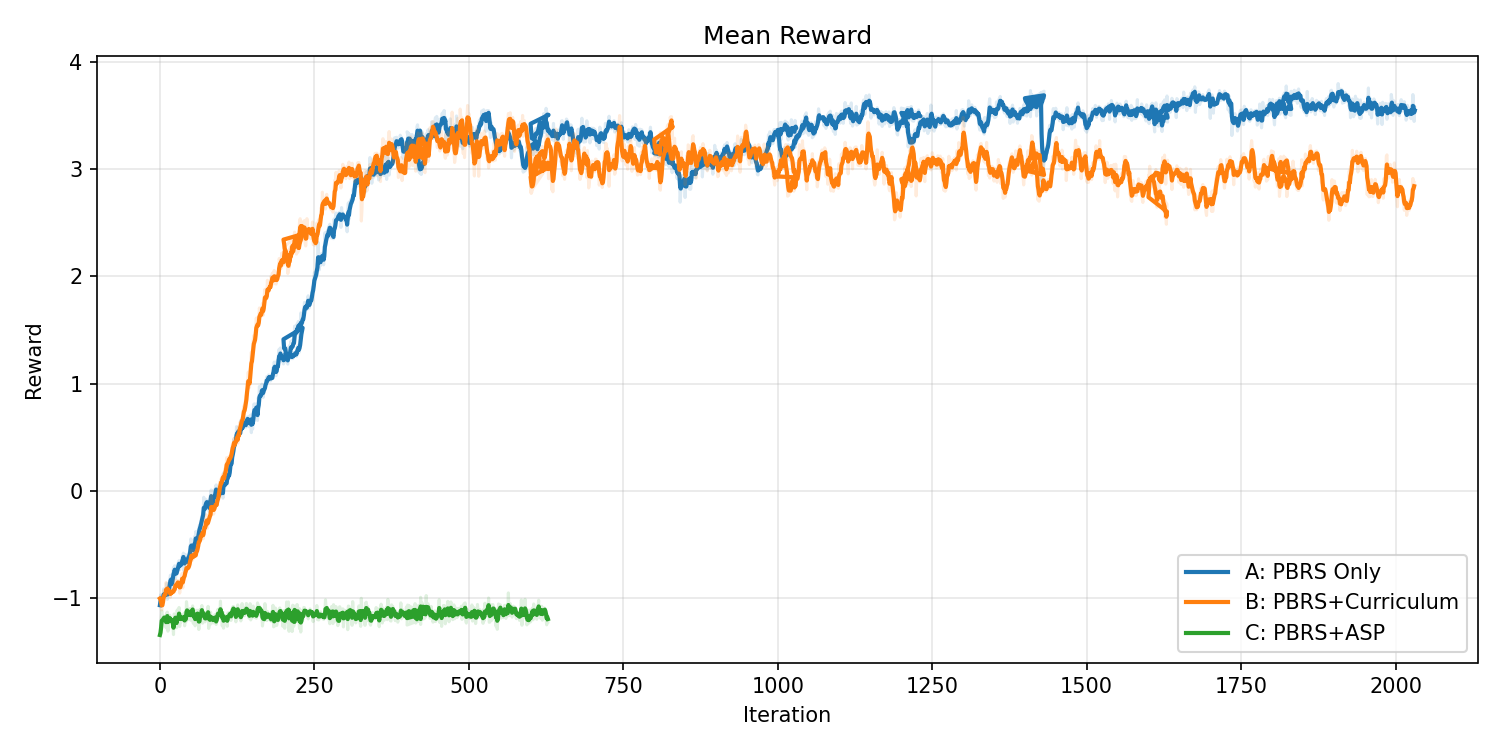
\includegraphics[width=0.72\textwidth]{figures/cmp_Mean_Reward.png}
    \end{column}
  \end{columns}

  \vspace{2pt}
  \begin{columns}[T]
    \begin{column}{0.48\textwidth}
      \centering
      \textbf{Policy Loss}
      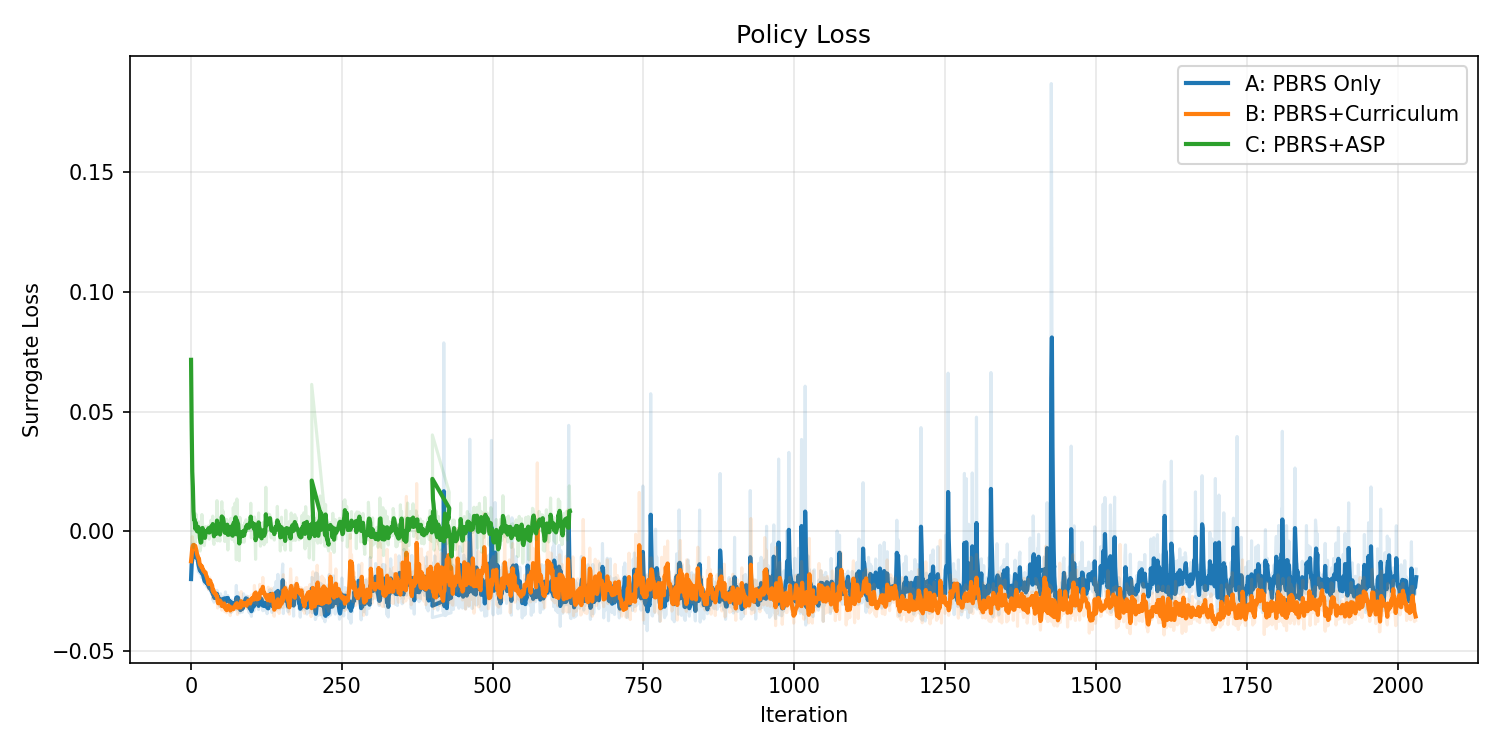
\includegraphics[width=0.72\textwidth]{figures/cmp_Policy_Loss.png}
    \end{column}
    \begin{column}{0.48\textwidth}
      \centering
      \textbf{Value Loss}
      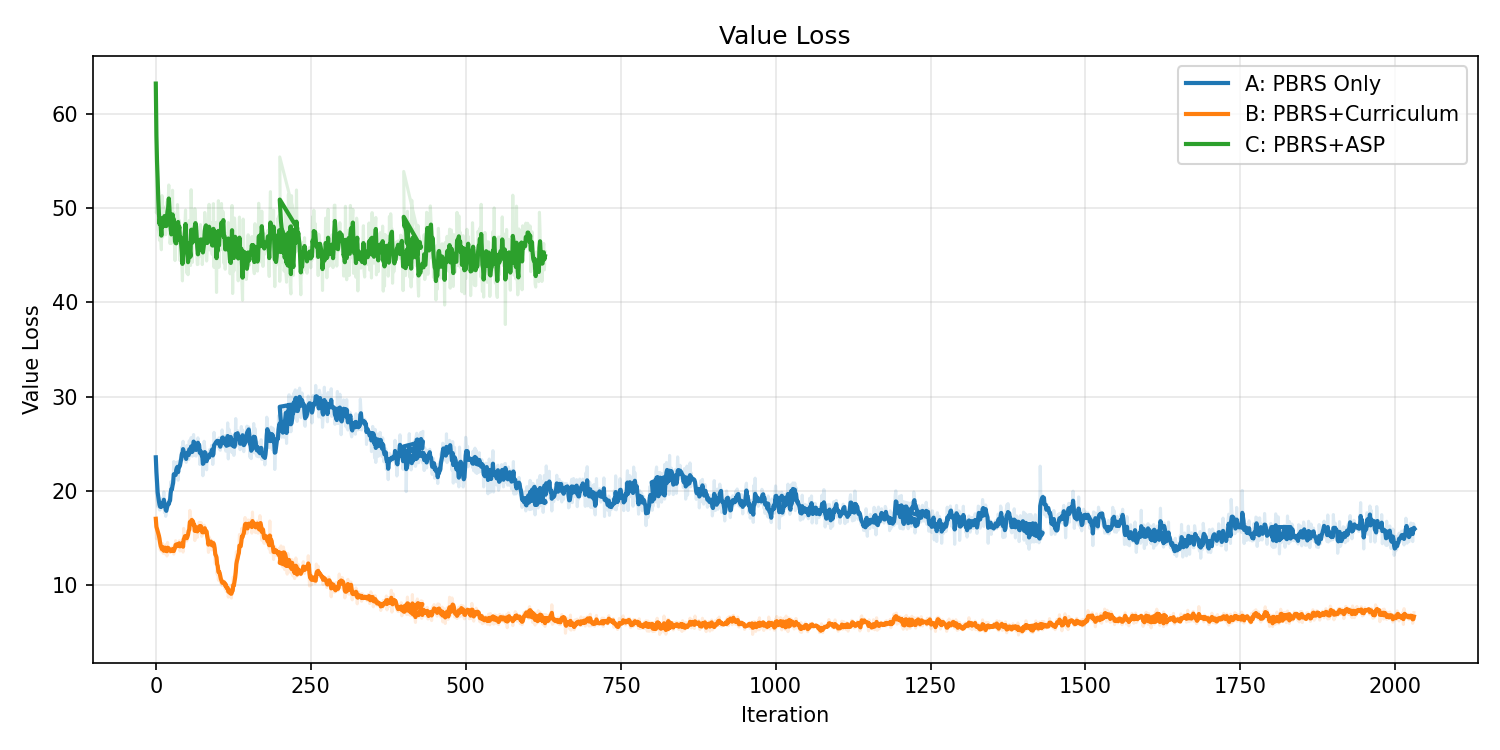
\includegraphics[width=0.72\textwidth]{figures/cmp_Value_Loss.png}
    \end{column}
  \end{columns}
\end{frame}

% --- Appendix C: PBRS theory analysis ---
\begin{frame}[t]{Appendix C — PBRS Theory Analysis}
  \begin{columns}[T]
    \begin{column}{0.48\textwidth}
      \centering
      \textbf{Potential Landscape} \\
      $\Phi(s) = w\cdot\exp(-k\cdot d^2)$
      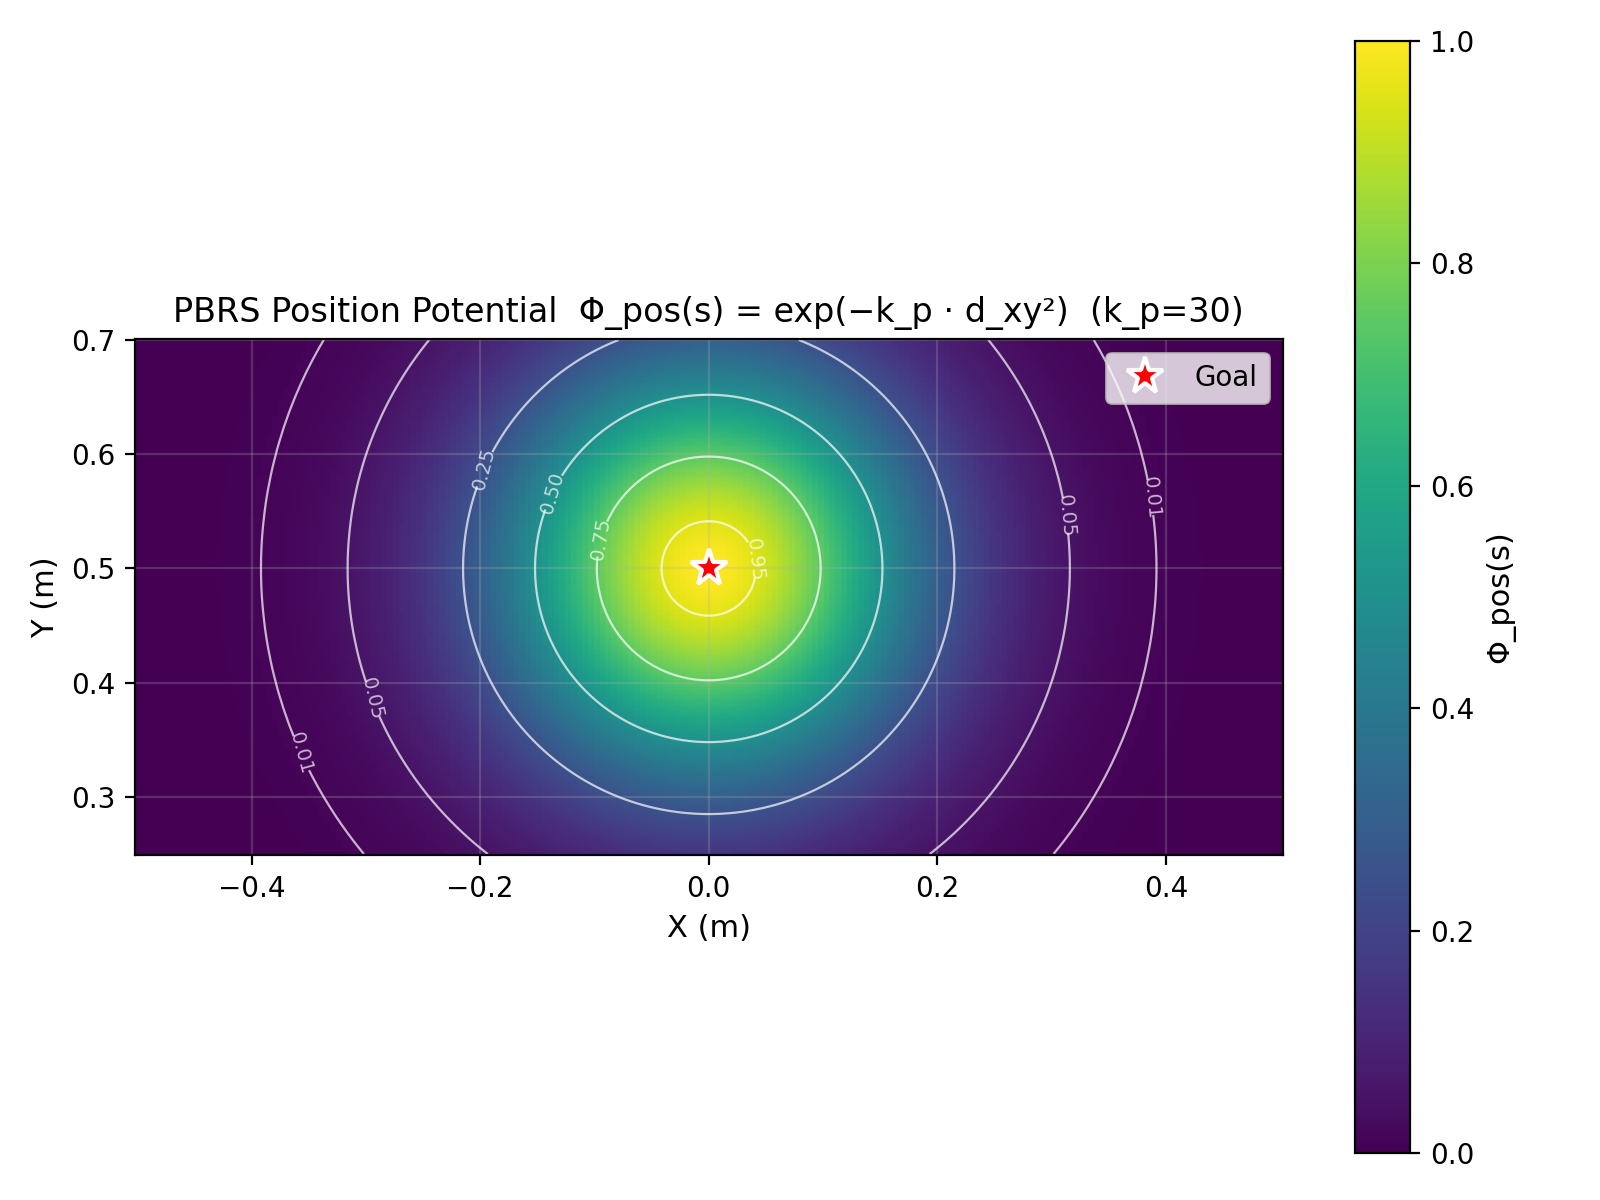
\includegraphics[width=0.52\textwidth]{figures/a1_potential_landscape.png}
    \end{column}
    \begin{column}{0.48\textwidth}
      \centering
      \textbf{Gradient Comparison} \\
      PBRS vs Fractional Formula
      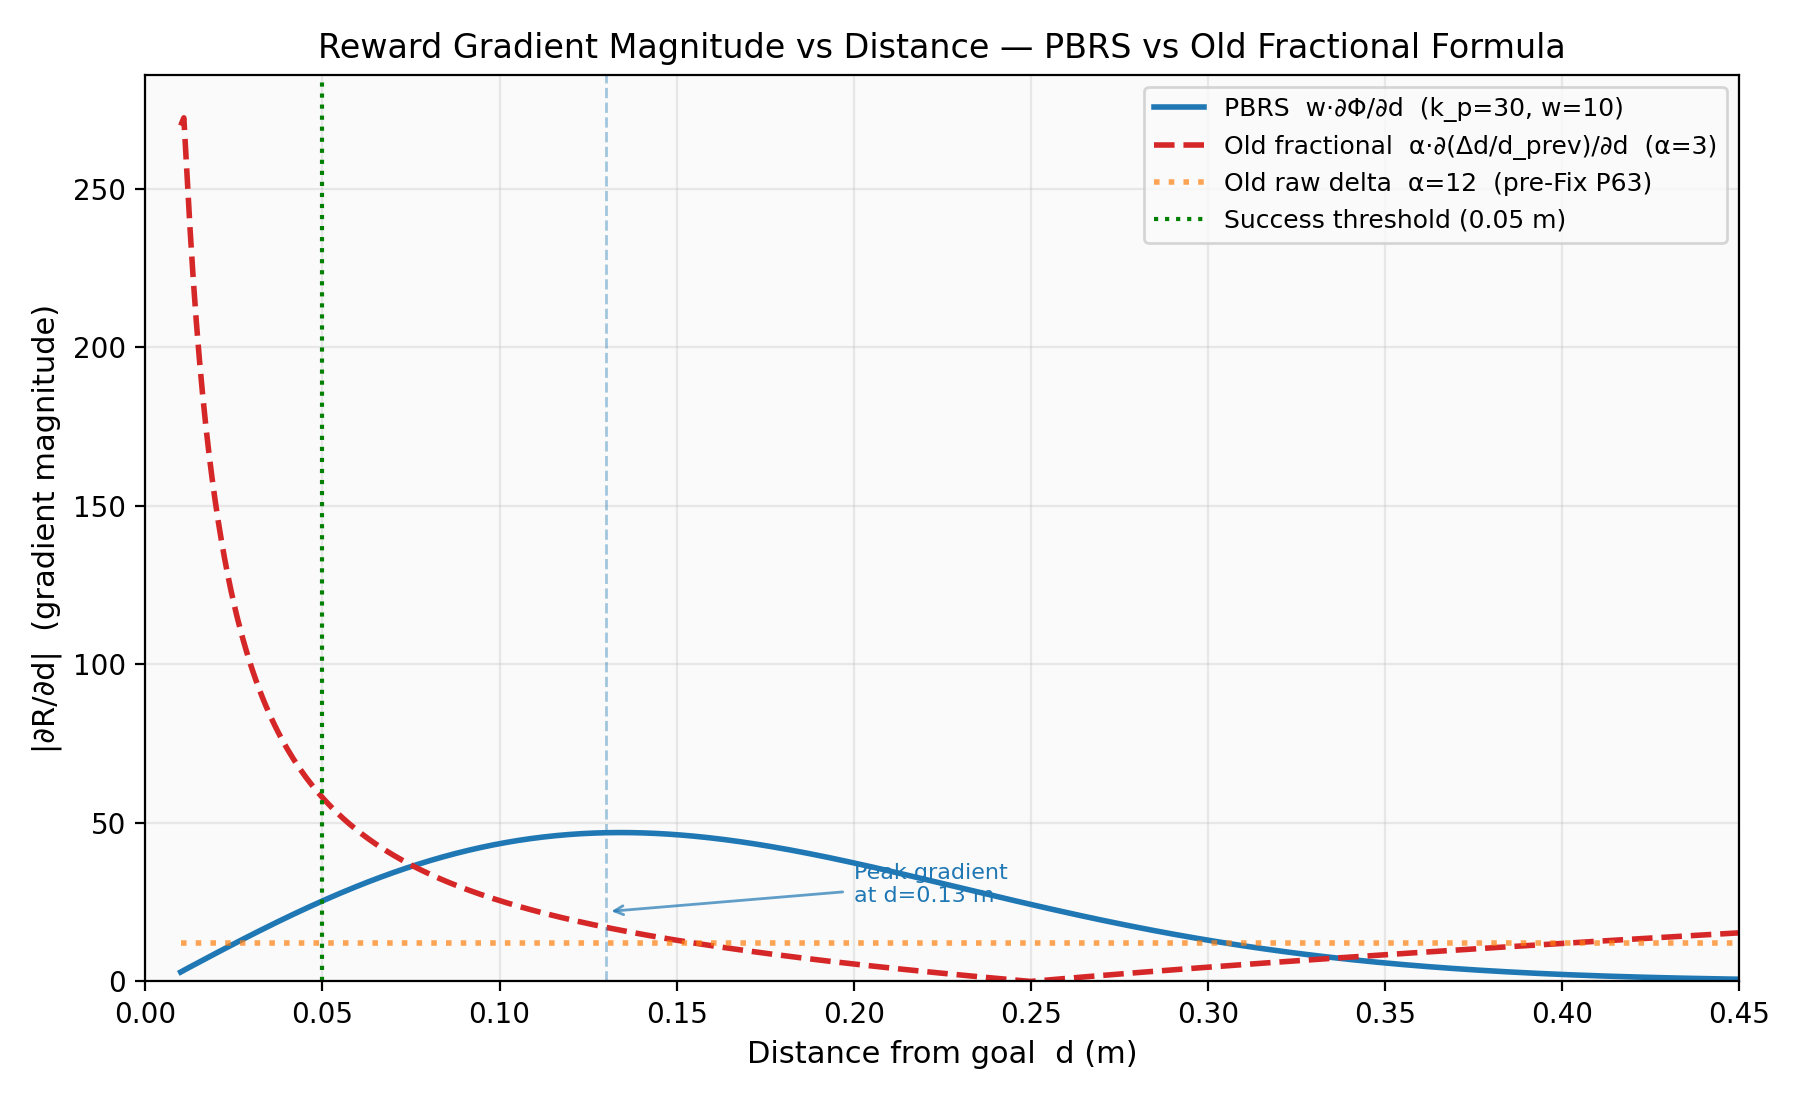
\includegraphics[width=0.52\textwidth]{figures/a2_gradient_comparison.png}
    \end{column}
  \end{columns}

  \vspace{2pt}
  \begin{center}
    \textbf{Cosine Angular Distance} $c(s) = (1-\cos(\theta^*-\theta))/2$
    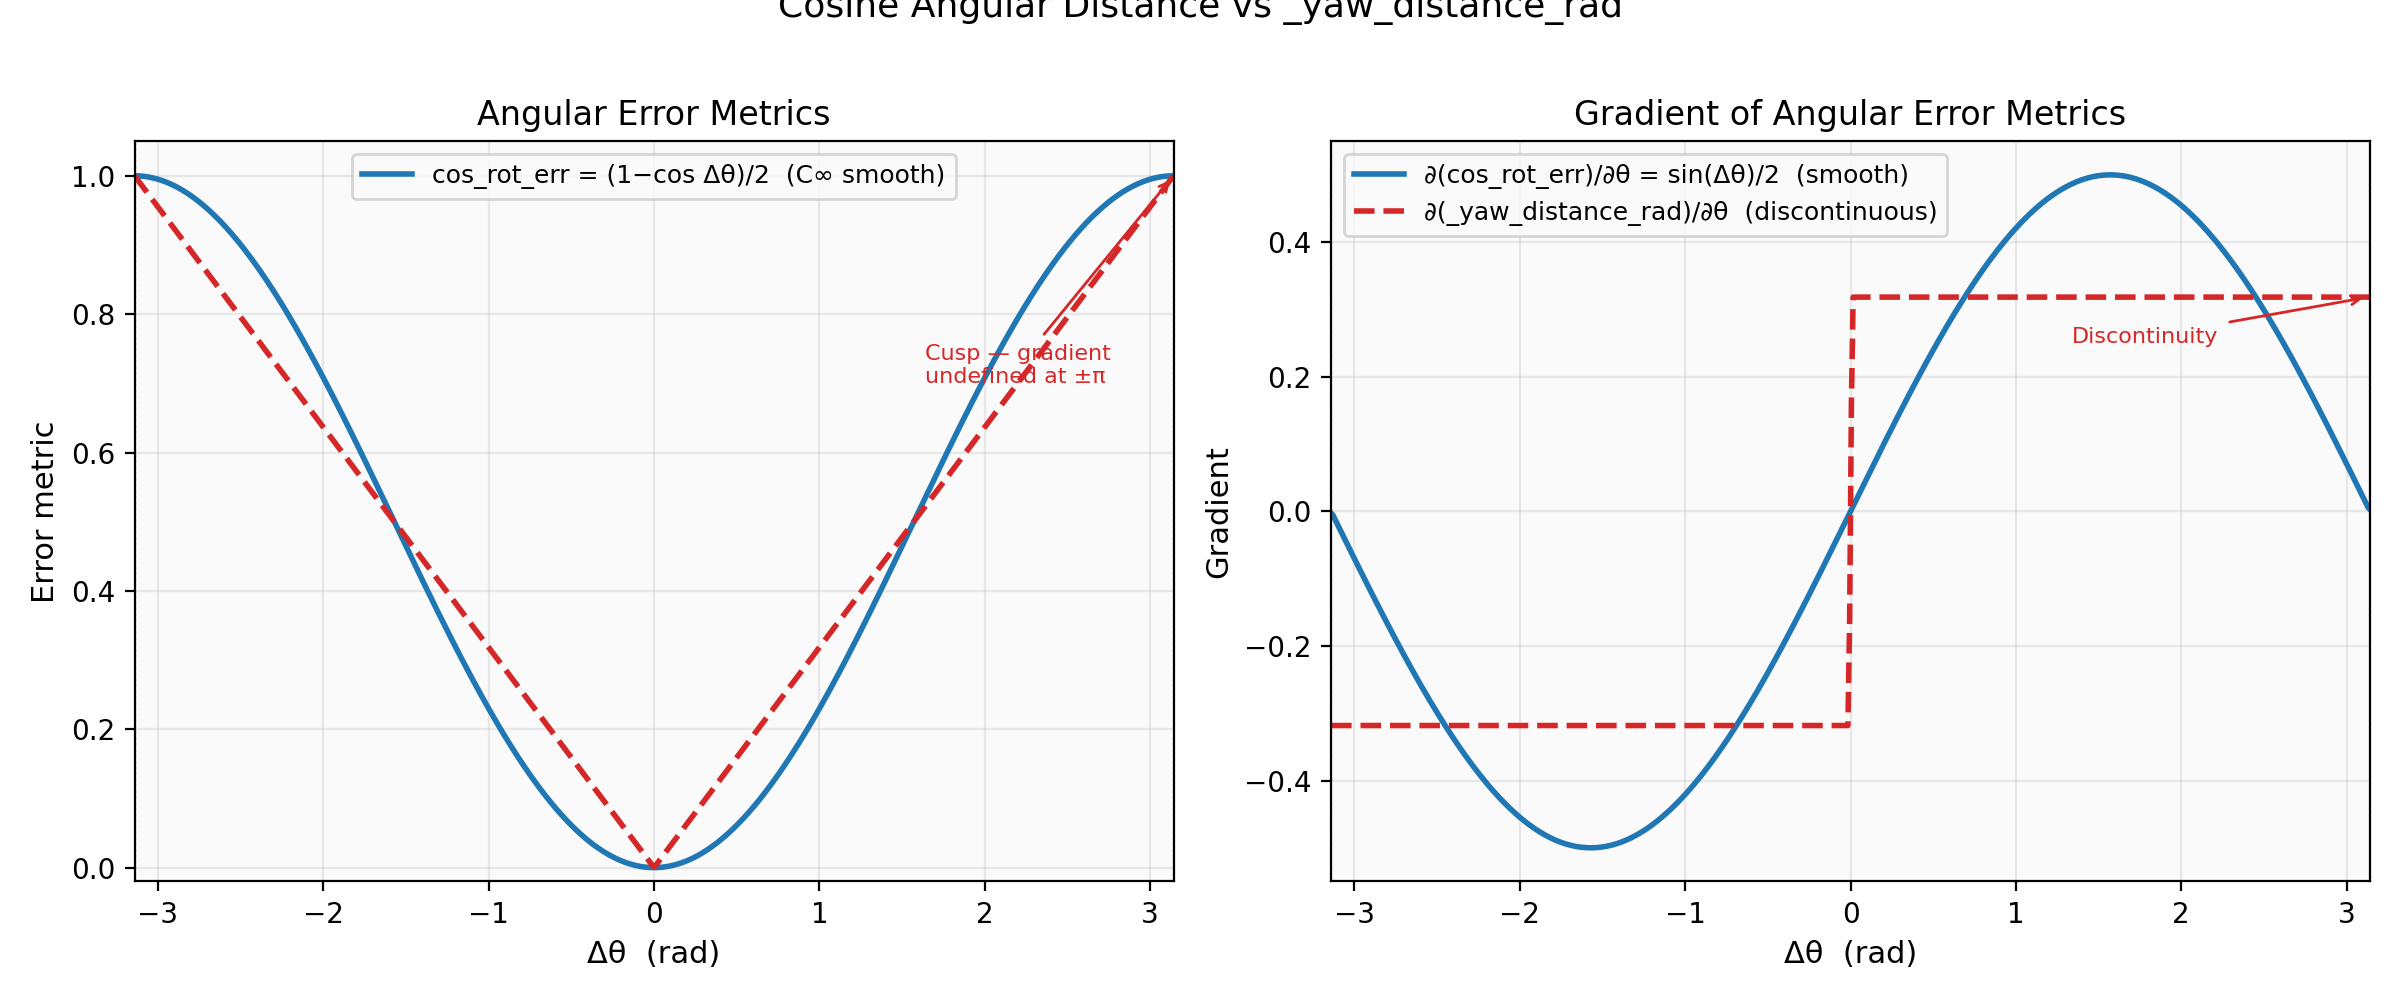
\includegraphics[width=0.30\textwidth]{figures/a4_cosine_distance.png}
  \end{center}
\end{frame}

% --- Appendix G: Per-test error bars (A vs B head-to-head + all models) ---
\begin{frame}[t]{Appendix G — Per-Test Error Bars (95\% Binomial CIs)}
  \centering
  
\includegraphics[width=0.85\textwidth]{figures/val_multi_error_bars.png}

  \vspace{6pt}
  {\small
  \textbf{Top:} A (blue) vs B (orange) head-to-head — per-scene trial-level SR from 20 trials. Overlapping CIs on most scenes.\\
  \textbf{Bottom:} All 6 models — ASP variants (E–H) are near-zero on all but the easiest scenes.\\
  \textbf{Green labels:} pos-only tests. \textbf{Purple labels:} pos+rot tests.
  }

  \vfill\litfooter{[Schulman et al.\ 2017]~[Ng et al.\ 1999]~[Grze\'s 2017]}
\end{frame}

\end{document}
